% Author: Sarthak Bhagwan Ingle | ID: 2022A7PS0037P
% Elsevier CAS double-column version generated from the revised manuscript.
\documentclass[a4paper,fleqn]{cas-dc}

\usepackage[numbers,sort&compress]{natbib}
\usepackage{amsmath,amssymb,amsfonts}
\usepackage{graphicx}
\usepackage{booktabs}
\usepackage{multirow}
\usepackage{url}
\usepackage[figuresright]{rotating}

\begin{document}
\let\WriteBookmarks\relax
\def\floatpagepagefraction{1}
\def\textpagefraction{.001}

\shorttitle{Continual-Mamba for IoT Intrusion Detection}
\shortauthors{Sarthak Bhagwan Ingle}

\title [mode = title]{Continual-Mamba for IoT Intrusion Detection: A Cross-Dataset Benchmark Study of Selective State Spaces, KAN Heads, and EWC under Task-Incremental Drift}

\author[1]{Sarthak Bhagwan Ingle}
\cormark[1]
\ead{f20220037@pilani.bits-pilani.ac.in}
\credit{Conceptualization, Methodology, Software, Experiments, Writing - original draft}

\affiliation[1]{organization={Department of Computer Science, BITS Pilani},
                city={Pilani},
                state={Rajasthan},
                country={India}}

\cortext[cor1]{Corresponding author}

\begin{abstract}
IoT intrusion detection in production networks is inherently non-stationary: models must adapt to new threats without silently losing prior attack knowledge. This paper identifies that continual IDS evaluation is first a protocol-validity problem: active-class logit masking and bounded class weighting are necessary preconditions for meaningful task-incremental measurement, because ignoring them can produce degenerate predictions and misleading retention-adaptation metrics under imbalanced attack-label drift. We study this issue with a compact IDS model that combines a selective state-space encoder, a KAN-inspired classifier head, and Elastic Weight Consolidation (EWC). We evaluate a two-phase task-incremental protocol on CIC-IoT2023 and repeat the same protocol on the independent ToN-IoT Network dataset. On CIC-IoT2023, single-seed controlled ablations compare Mamba+KAN, Mamba+MLP, and MLP+KAN variants with and without EWC, plus a 34-class full-label reference run and a joint-training upper bound. The best single-seed reduced-protocol setting (Mamba+KAN+EWC(5)) achieves Phase-1-after-Phase-2 accuracy 58.46\%, Phase-2 accuracy 98.29\%, and average accuracy $A_k$ 78.38\%, improving $A_k$ by 0.54 points over Mamba+KAN without EWC; however, a new three-seed rerun of the main Mamba+KAN pair shows high variance and does not support a robust EWC(5) superiority claim. Under full 34-class evaluation, $A_k$ decreases to 69.08\%, and a 12-epoch joint-training upper bound reaches $A_k=89.79\%$, quantifying the remaining continual-learning gap. On ToN-IoT, Mamba+KAN with light EWC(0.2) improves $A_k$ from 80.60\% to 81.54\% over sequential finetuning. A same-dataset CIC-IDS2017 static check reaches 97.92\% weighted F1 versus the MAMBA--KAN reference's reported 96.54\% CICIDS2017 F1, while macro-F1 remains 69.44\% because of rare classes. Across the reported continual datasets, backward transfer remains negative, so the contribution is a security-facing evaluation protocol, reproducible benchmark evidence, and a bounded retention improvement rather than a complete solution to catastrophic forgetting.
\end{abstract}

\begin{highlights}
\item Identifies active-class logit masking and bounded class weighting as necessary protocol conditions for valid continual IDS evaluation.
\item Benchmarks compact Mamba-style and KAN-inspired IDS variants under CIC-IoT2023 and ToN-IoT task-incremental drift.
\item Reports robustness limits, a joint-training upper bound, and rare-class macro-F1 limitations for deployment-facing interpretation.
\end{highlights}

\begin{keywords}
continual learning \sep intrusion detection \sep Mamba \sep Kolmogorov-Arnold Networks \sep EWC \sep CIC-IoT2023 \sep CIC-IDS2017 \sep ToN-IoT
\end{keywords}

\maketitle
\section{Introduction}
Intrusion Detection Systems (IDS) for IoT environments operate under persistent distribution drift: new attack families emerge, class frequencies shift, and traffic semantics evolve over time. In this setting, a model update process must satisfy two conflicting objectives: \textit{plasticity} (learning new patterns quickly) and \textit{stability} (retaining old patterns). Standard finetuning often optimizes plasticity at the cost of catastrophic forgetting.

Before comparing architectures or continual-learning algorithms, an IDS update benchmark must first ensure that its protocol is valid for the security question being asked. In task-incremental IDS evaluation, only a subset of attack labels is active during a given update phase. If the loss or prediction rule allows inactive labels to compete with active ones, the resulting accuracy can reflect protocol artifacts rather than real attack retention. Similarly, unbounded inverse-frequency weighting can let tiny rare-class counts dominate optimization. We therefore treat active-class logit masking and bounded class weighting as necessary preconditions for valid continual IDS measurement, not as minor implementation details.

Recent IDS work has shown promise from state-space sequence models and KAN-style nonlinear heads for efficient representation and classification. A Mamba--KAN IDS combination has also been studied in a static setting~\cite{zhao2025}, where the reported F1 scores are high under conventional train/test evaluation. However, most prior pipelines are evaluated using static splits and do not explicitly quantify forgetting under sequential task exposure. This motivates a continual-learning benchmark where architecture quality, update strategy, and task protocol are reported separately. In this framing, Mamba+KAN+EWC(5) is evaluated as a retention mechanism for an already competitive architecture, not as a direct static replacement for prior Mamba--KAN results.

This paper makes five empirical contributions:
\begin{itemize}
\item A protocol-validity finding for continual IDS: active-class logit masking and bounded class weighting are required to avoid invalid retention-adaptation measurements under task-incremental label drift.
\item A reproducible task-incremental IDS benchmark on CIC-IoT2023 and ToN-IoT, including retention, adaptation, forgetting, macro-F1, latency, multi-seed checks, and a joint-training upper bound.
\item A controlled architecture-vs-continual-learning comparison across Mamba+KAN, Mamba+MLP, and MLP+KAN variants, with no-EWC and EWC settings.
\item A same-dataset static CIC-IDS2017 check against the MAMBA--KAN reference paper, where the local Mamba+KAN implementation reaches 97.92\% weighted F1 compared with the reference's reported 96.54\% CICIDS2017 F1, while exposing a 69.44\% macro-F1 rare-class limitation.
\item An extended N-task implementation with LwF, ER/ER-ACE/DER++ replay, joint-training upper bounds, class-frequency-aware Fisher weighting, and multi-seed reporting support for follow-up evaluation.
\end{itemize}

\section{Related Work}
\subsection{Intrusion Detection Architectures}
Traditional IDS methods rely on engineered features with classical learners (SVM, RF, XGBoost). Deep models expanded representational power via CNNs, RNNs, and Transformers, but controlled comparisons remain difficult because NIDS papers often differ in datasets, preprocessing, metrics, and train/test protocols~\cite{gamage2020survey}. Transformer variants capture long-range interactions but scale quadratically in sequence length, challenging edge deployment constraints.

State-space models, including selective variants, offer linear-time sequence processing and improved hardware efficiency. KAN formulations replace fixed MLP activations with learnable basis-function compositions and have shown competitive approximation behavior with compact parametrization.

\subsection{Continual Learning in Classification}
Continual-learning approaches can be grouped into replay-based, regularization-based, and parameter-isolation methods. EWC is a regularization approach that penalizes movement of parameters with high Fisher importance to previous tasks. Related methods include Synaptic Intelligence (SI), Memory Aware Synapses (MAS), and Learning without Forgetting (LwF).

Replay-based methods such as experience replay, ER-ACE, and DER++ and parameter-isolation methods such as PackNet are stronger continual-learning baselines than EWC alone, particularly when memory or task-specific subnetworks are allowed. Distillation methods such as LwF provide a memory-free baseline by matching the previous model's softened logits during new-task training. The full reported benchmark keeps its main comparison focused on compact regularization-based updates, but the released implementation now includes LwF, ER, ER-ACE-style replay, DER++-style replay, and a joint-training upper-bound runner for larger follow-up experiments. PackNet remains a future parameter-isolation baseline.

\subsection{Continual Learning for IDS}
Recent IDS-specific continual-learning work has begun to move beyond static train/test evaluation. CITADEL studies continual anomaly detection for IoT IDS and combines self-supervised representation learning with memory consolidation and novelty detection~\cite{li2025citadel}. SSF addresses concept drift in network intrusion detection through strategic sample selection and forgetting with a refreshed memory buffer~\cite{zhang2025ssf}. SOUL studies semi-supervised open-world continual learning for NID, emphasizing label scarcity, replay, and attack-class performance decay over time~\cite{amalapuram2024soul}. Incremental IDS systems based on active learning and sliding-window retraining similarly motivate adaptive security evaluation, although they do not isolate the same task-incremental masking and class-weighting issue studied here~\cite{boukela2023incremental}. Relative to this emerging literature, this paper focuses on protocol validity for task-incremental multi-class IDS and reports architecture, regularization, upper-bound, and multi-seed checks in one reproducible pipeline.

\section{Problem Formulation}
Let $\mathcal{D}_1,\ldots,\mathcal{D}_T$ denote sequential tasks sampled from evolving traffic distributions. The model learns task $k$ after tasks $1,\ldots,k-1$ without full joint retraining on all previous data. Each task has an active label set $\mathcal{C}_k$, and the model has a single classifier over the union $\mathcal{C}=\cup_{k=1}^{T}\mathcal{C}_k$.

This work uses a task-incremental setting: the phase identity, and therefore $\mathcal{C}_k$, is known during training and evaluation. For an example $(x,y)$ from task $k$, logits outside $\mathcal{C}_k$ are excluded from the supervised loss and task-aware prediction:
\begin{equation}
\ell_k(x,y)=\text{CE}(f_\theta(x)_{\mathcal{C}_k}, \pi_k(y)),
\end{equation}
where $\pi_k$ maps the global label index to its local index inside $\mathcal{C}_k$. This protocol is less general than open class-incremental IDS, but it is appropriate when an update is deployed for a known attack phase or labeled monitoring interval.

For model $f_\theta$, define:
\begin{itemize}
\item $a_{k,t}$: Task-$t$ accuracy after training has completed through task $k$.
\item $a_{t,t}$: Task-$t$ accuracy immediately after learning task $t$.
\item $a_{T,t}$: Task-$t$ accuracy at the end of the stream.
\end{itemize}

Primary metrics are:
\begin{equation}
A_k = \frac{1}{k}\sum_{t=1}^{k} a_{k,t}
\end{equation}
\begin{equation}
\text{BWT}_T = \frac{1}{T-1}\sum_{t=1}^{T-1}(a_{T,t}-a_{t,t})
\end{equation}
Negative BWT indicates forgetting. The earlier two-phase results are the special case $T=2$, where $\text{BWT}=a_{2,1}-a_{1,1}$.

\section{Dataset and Protocol}
\subsection{Datasets}
The primary benchmark uses CIC-IoT2023 merged CSV files with 39 engineered network-flow features and multi-class attack labels~\cite{ciciot2023}. We use two CIC-IoT2023 evaluation regimes:
\begin{itemize}
\item Reduced protocol: 13-class union for controlled ablations.
\item Full protocol: 34-class union for realistic benchmark stress.
\end{itemize}

As an external sanity check, we also evaluate on the independent ToN-IoT Network dataset~\cite{toniot2020}. The downloaded network CSV contains 211,043 records and 10 traffic types: normal, ddos, dos, scanning, injection, xss, password, backdoor, ransomware, and mitm. After preprocessing, the ToN-IoT experiment uses 35 numeric features and the multi-class \texttt{type} field as the target.

For a same-dataset comparison with the MAMBA--KAN reference paper, we additionally run a static CIC-IDS2017 experiment using the local day-wise CSV files. The static check contains 2,830,743 rows, 78 numeric features after identifier removal, and 15 attack/benign labels.

\subsection{Task Construction}
CIC-IoT2023 task partitioning follows semantic attack groups:
\begin{itemize}
\item \textbf{Phase-1}: benign and flooding-dominant classes.
\item \textbf{Phase-2}: benign plus Mirai/recon/application attack classes.
\end{itemize}

For ToN-IoT, the external validation split is:
\begin{itemize}
\item \textbf{Phase-1}: normal, ddos, dos, and scanning.
\item \textbf{Phase-2}: normal, injection, xss, password, backdoor, ransomware, and mitm.
\end{itemize}

For follow-up scalability experiments, the implementation now also supports an arbitrary ordered task list. A checked 4-task CIC-IoT2023 stream separates DDoS flooding, DoS/fragmentation, Mirai/reconnaissance, and web/spoofing/malware groups. The small run reported later is used only to validate the extended pipeline; the main quantitative claims in this draft still come from the full two-phase experiments in Tables~\ref{tab:mainbench} and~\ref{tab:toniot}.

\subsection{Data Split and Preprocessing}
CIC-IoT2023 merged files are split by file order into train/validation/test (80/10/10). For ToN-IoT, the single public network CSV is converted into ten stratified \texttt{Merged*.csv} shards and then split by file order into train/validation/test (70/10/20). The CIC-IDS2017 static check uses a stratified 80/10/10 split across all local rows so that minority labels appear in the evaluation split. Preprocessing includes:
\begin{enumerate}
\item numeric conversion with NaN/inf sanitization,
\item clipping to bounded numeric range,
\item categorical encoding for ToN-IoT protocol/service/state fields,
\item removal of direct identifiers and the binary \texttt{label} column to avoid leakage into multi-class \texttt{type} prediction,
\item feature standardization fitted on Phase-1 train only.
\end{enumerate}

\section{Method}
\subsection{Architecture}
The model has three components:
\begin{enumerate}
\item \textbf{Tokenized feature encoder}: feature vector reshaped into short token sequence.
\item \textbf{Backbone}: selective SSM blocks (Mamba-style) or feed-forward baseline.
\item \textbf{Classifier head}: KAN-inspired basis head or MLP baseline.
\end{enumerate}

\subsection{Selective SSM Update}
For hidden state $h_t$ and token input $x_t$:
\begin{equation}
h_t = (1 + \Delta_t A)h_{t-1} + \Delta_t \odot g_t \odot Ux_t
\end{equation}
\begin{equation}
y_t = Wh_t
\end{equation}
where $\Delta_t$ and $g_t$ are input-dependent step and gate terms.

\subsection{KAN-Inspired Head}
For input vector $x\in\mathbb{R}^{d}$, basis activations are radial components:
\begin{equation}
\phi_{i,j}(x_i)=\exp\left(-\left(\frac{x_i-c_{i,j}}{\sigma_{i,j}}\right)^2\right)
\end{equation}
with learnable centers $c_{i,j}$ and widths $\sigma_{i,j}$. The output is
\begin{equation}
\hat{y}=W_{\phi}\Phi(x)+W_b x
\end{equation}
which combines basis expansion and linear shortcut.

\subsection{Continual Objective with EWC}
For task $k>1$, the EWC objective is:
\begin{equation}
\mathcal{L}=\mathcal{L}_{\text{CE}}+\frac{\lambda}{2}\sum_i F_i(\theta_i-\theta_i^*)^2
\end{equation}
where $F_i$ is diagonal Fisher information from prior tasks.

For imbalanced IoT labels, the implementation also supports a class-frequency-aware Fisher estimate:
\begin{equation}
F_i^{\text{CFA}}=\mathbb{E}_{(x,y)\sim\mathcal{D}_k}
\left[w_y\left(\frac{\partial \log p_\theta(y|x)}{\partial\theta_i}\right)^2\right],
\end{equation}
where $w_y$ is a bounded inverse-square-root class-frequency weight. This gives rare but security-relevant attack classes more influence in the consolidation penalty without allowing extreme weights to dominate optimization. Full-scale evaluation of this variant is left to the extended benchmark runs.

\subsection{Distillation and Replay Extensions}
The extended implementation includes LwF and replay baselines for follow-up experiments. For LwF, a frozen teacher $f_{\theta^-}$ from the previous task regularizes the current model using softened logits:
\begin{equation}
\mathcal{L}_{\text{LwF}}=T^2\text{KL}\left(
\sigma(f_{\theta^-}(x)/T)\,\|\,\sigma(f_\theta(x)/T)
\right).
\end{equation}
For ER and DER++-style baselines, a class-balanced exemplar buffer stores old samples; DER++ additionally stores old logits and adds a mean-squared logit matching loss. ER-ACE-style runs keep the active-class current-task loss while replaying old examples over the union label space.

\subsection{Phase-Aware Class Masking}
A crucial stabilization is restricting logits to active classes for each phase. In implementation, the output layer always spans the union label space, but the loss and task-aware evaluation select only the current phase's active classes:
\begin{equation}
\hat{y}_k=\mathcal{C}_k\left[\arg\max_j z_{\mathcal{C}_k,j}\right].
\end{equation}
This is not a post-hoc metric adjustment: the same active-set selection is used during both optimization and evaluation. Without it, inactive logits from unseen or irrelevant classes can dominate the softmax and produce invalid predictions under task-incremental labels. The assumption is that the active task is known; removing this assumption is left to class-incremental future work.

\section{Experimental Settings}
\subsection{Hardware and Software}
All experiments were run on a single consumer-grade laptop platform: NVIDIA RTX 3050 Laptop GPU (4GB), Intel i7-12700H CPU, 16GB RAM, and PyTorch 2.3.1 with CUDA 12.1. Reporting this environment is important for two reasons. First, the paper targets practical IDS update settings where full retraining may be constrained by available compute. Second, the compact model width, batch size, and sample caps were chosen to fit this hardware, so the reported latency and scalability claims should be interpreted as local measurements rather than hardware-independent constants.

\subsection{Benchmark Matrix}
We compare:
\begin{itemize}
\item CIC-IoT2023 reduced protocol: Mamba+KAN, Mamba+MLP, and MLP+KAN with and without EWC.
\item CIC-IoT2023 full protocol: one 34-class Mamba+KAN reference run.
\item ToN-IoT external validation: Mamba+KAN with an EWC sensitivity sweep.
\item Extended implementation validation: a 4-task CIC-IoT2023 smoke stream with LwF, ER+EWC, DER++ + EWC, a joint-training upper-bound runner, ER-ACE-style replay support, class-frequency-aware Fisher support, and a two-seed summary.
\end{itemize}

\subsection{Hyperparameter Summary}
All reported runs use the same hardware stack. The two main reduced Mamba+KAN settings include a three-seed robustness check; the other architecture variants, ToN-IoT sweep, full34 reference, and static CIC-IDS2017 check remain point estimates unless explicitly marked otherwise.

\begin{table}[htbp]
\caption{Core Hyperparameters}
\label{tab:hyp}
\centering
\begin{tabular}{lc}
\toprule
Parameter & Value \\
\midrule
Batch size & 256 \\
Epochs (Phase-1, Phase-2) & 6, 6 \\
Learning rate & 8e-4 \\
Weight decay & 1e-4 \\
Label smoothing & 0.05 \\
SSM layers & 2 \\
Model width $d_{model}$ & 96 \\
KAN hidden / grid & 96 / 8 \\
EWC $\lambda$ (CIC) & 0, 5, 40 \\
EWC $\lambda$ (ToN) & 0, 0.2, 1, 5 \\
Replay buffer (smoke) & 1000 exemplars \\
\bottomrule
\end{tabular}
\end{table}

\section{Results}
\subsection{CIC-IoT2023 Benchmark}
This subsection reports the main controlled CIC-IoT2023 evidence. The reduced protocol isolates architecture and continual-learning behavior on a 13-class union, while the full34 row stress-tests the same modeling approach under the broader label space. The joint-training row is not a continual-learning method; it is an upper bound obtained by retraining on the union of the reduced-protocol task data, and therefore quantifies how much performance is lost when the model is forced to update sequentially rather than jointly.

\begin{table*}[htbp]
\caption{CIC-IoT2023 Controlled Continual Benchmark (Reduced Protocol + Full34 Reference)}
\label{tab:mainbench}
\centering
\begin{tabular}{lcccccccc}
\toprule
Run & P1 Before & P1 After & P2 After & BWT & $A_k$ & P1 Macro-F1 & P2 Macro-F1 & Classes \\
\midrule
Mamba+KAN / No-EWC & 80.45 & 57.34 & 98.34 & -23.11 & 77.84 & 43.11 & 52.46 & 13 \\
Mamba+KAN / EWC(5) & 80.45 & 58.46 & 98.29 & -21.99 & 78.38 & 43.35 & 53.88 & 13 \\
Joint upper / Mamba+KAN & -- & 80.77 & 98.80 & -- & 89.79 & 76.32 & 54.37 & 13 \\
Mamba+MLP / No-EWC & 80.81 & 47.50 & 84.47 & -33.31 & 65.99 & 35.46 & 44.43 & 13 \\
Mamba+MLP / EWC(5) & 80.81 & 54.81 & 98.56 & -25.99 & 76.69 & 46.23 & 52.68 & 13 \\
MLP+KAN / No-EWC & 79.98 & 47.78 & 97.44 & -32.20 & 72.61 & 43.01 & 48.75 & 13 \\
MLP+KAN / EWC(5) & 79.98 & 35.34 & 98.16 & -44.64 & 66.75 & 31.55 & 49.15 & 13 \\
Full34 / Mamba+KAN EWC(20) & 77.43 & 53.73 & 84.42 & -23.70 & 69.08 & 34.76 & 37.49 & 34 \\
\bottomrule
\end{tabular}
\end{table*}

\begin{table}[htbp]
\caption{Three-Seed Robustness Check for Reduced Mamba+KAN Runs (Mean $\pm$ Std., \%)}
\label{tab:main-multiseed}
\centering
\scriptsize
\begin{tabular}{lcccc}
\toprule
Run & P1 After & P2 After & BWT & $A_k$ \\
\midrule
No-EWC & $35.07\pm5.34$ & $91.39\pm9.90$ & $-44.94\pm4.77$ & $63.23\pm5.78$ \\
EWC(5) & $33.73\pm15.00$ & $85.20\pm11.93$ & $-46.28\pm14.28$ & $59.47\pm5.94$ \\
\bottomrule
\end{tabular}
\end{table}

\subsection{CIC-IoT2023 Table-Level Inference}
Table~\ref{tab:mainbench} and Table~\ref{tab:main-multiseed} show four important patterns.
\begin{itemize}
\item \textbf{Protocol design is the first result:} active-class masking and bounded class weighting are required before BWT and $A_k$ can be interpreted as security-relevant retention metrics.
\item \textbf{Single-seed EWC gains are not robust:} the original point estimate for Mamba+KAN+EWC(5) improves BWT and $A_k$, but the new three-seed rerun shows high variance and lower mean performance for EWC(5) than no-EWC. Therefore, the defensible claim is protocol validity plus bounded point-estimate improvement, not statistical EWC superiority.
\item \textbf{Architecture and CL are coupled:} EWC benefit is variant dependent (helpful for Mamba+MLP, harmful for MLP+KAN at same $\lambda$), so CL regularization must be tuned per backbone/head combination.
\item \textbf{The continual gap is large:} the 12-epoch joint-training upper bound reaches $A_k=89.79\%$, while the best sequential reduced point estimate is $78.38\%$ and the three-seed sequential means are lower. Moving from 13 to 34 classes further reduces adaptation and macro-F1.
\end{itemize}

\subsection{Direct Comparison to the MAMBA--KAN Reference}
The closest architectural inspiration, MAMBA--KAN for static network intrusion detection~\cite{zhao2025}, reports strong single-split classification results, including F1 scores of 99.90\% on CIC-IoT2022, 96.54\% on CICIDS2017, 99.69\% on USTC-TFC2016, and 91.64\% on CrossPlatform(Android). These numbers show that the MAMBA--KAN architecture is already competitive in conventional static IDS evaluation. However, those results are not a direct head-to-head comparison with Table~\ref{tab:mainbench}, because the reference paper does not evaluate sequential task exposure, Phase-1 retention after Phase-2 learning, backward transfer, or $A_k$.

\begin{table*}[htbp]
\caption{Defensible Comparison with the Static MAMBA--KAN Reference}
\label{tab:prior-context}
\centering
\small
\begin{tabular}{p{0.18\textwidth}p{0.24\textwidth}p{0.31\textwidth}p{0.18\textwidth}}
\toprule
Question & MAMBA--KAN reference~\cite{zhao2025} & This work & Precise claim \\
\midrule
Raw static IDS classification & Static F1: 99.90\% on CIC-IoT2022, 96.54\% on CICIDS2017, 99.69\% on USTC-TFC2016, and 91.64\% on CrossPlatform(Android). & Not a matched static rerun; the main metrics are continual $A_k$, BWT, and post-update task accuracies on CIC-IoT2023 and ToN-IoT. & Do not claim universal static SOTA. \\
Sequential update behavior & Not reported. & CIC-IoT2023 reduced protocol: Phase-1-after-Phase-2 accuracy 58.46\%, Phase-2 accuracy 98.29\%, BWT $=-21.99$, and $A_k=78.38\%$ in the best single-seed EWC point estimate. & Adds continual-learning evidence absent from the reference. \\
Benefit over the same Mamba+KAN architecture & No EWC or forgetting comparison. & In the original single-seed pair, EWC(5) improves Phase-1-after accuracy by 1.12 points, BWT by 1.12 points, $A_k$ by 0.54 points, and Phase-2 macro-F1 by 1.42 points. A three-seed rerun does not confirm robust EWC(5) superiority. & Point-estimate improvement, not statistical superiority. \\
External continual validation & Four static datasets; no ToN-IoT continual stream. & On ToN-IoT, EWC(0.2) improves $A_k$ from 80.60\% to 81.54\% and Phase-2 macro-F1 from 86.25\% to 88.00\% over no-EWC. & Same retention-adaptation pattern appears on a second IDS corpus. \\
Benchmark scope & Static train/test comparison with MAMBA-only and KAN-only ablations. & Architecture-vs-continual-learning ablations, a full 34-class stress run, active-class masking, and extended N-task/replay implementation paths. & More complete continual IDS benchmark. \\
\bottomrule
\end{tabular}
\end{table*}

Therefore, the appropriate answer to the reference-paper comparison is not that Mamba+KAN+EWC(5) universally exceeds prior static IDS classifiers in raw F1. Rather, this work contributes a continual-update evaluation protocol that the static reference does not study. In the original single-seed CIC-IoT2023 pair, EWC(5) improves Phase-1-after accuracy by 1.12 percentage points, improves BWT by 1.12 points, increases $A_k$ by 0.54 points, and raises Phase-2 macro-F1 by 1.42 points relative to no-EWC, while preserving high Phase-2 adaptation (98.29\% versus 98.34\%). However, the three-seed rerun in Table~\ref{tab:main-multiseed} shows that this EWC(5) advantage is not robust under the current runner. The stronger and more stable claim is that the paper identifies protocol conditions required for valid continual IDS evaluation, quantifies the gap to joint retraining, and exposes where compact EWC regularization is insufficient. A broader static state-of-the-art claim would require matched static re-runs on the same datasets, labels, preprocessing, and train/test protocol.

\subsection{Same-Dataset Static Check on CICIDS2017}
To make the comparison more concrete, the local Mamba+KAN implementation was also evaluated on the CIC-IDS2017 CSV files used in many IDS studies and reported in the MAMBA--KAN reference. The experiment uses all 2,830,743 local rows, 78 numeric features after identifier removal, 15 labels, and a stratified 80/10/10 split. Training used the same compact Mamba+KAN variant for five epochs with class weighting and label smoothing. Table~\ref{tab:cicids2017-static-check} compares the local result against the CICIDS2017 rows reported by Zhao and Zhang~\cite{zhao2025}.

\begin{table*}[htbp]
\caption{Same-Dataset CICIDS2017 Static Comparison Against the MAMBA--KAN Reference}
\label{tab:cicids2017-static-check}
\centering
\begin{tabular}{lccccc}
\toprule
Method & Average & Accuracy & Precision & Recall & F1 \\
\midrule
RF~\cite{zhao2025} & reported & 99.83 & 90.59 & 87.32 & 88.92 \\
CNN~\cite{zhao2025} & reported & 99.79 & 89.35 & 82.56 & 85.82 \\
LSTM~\cite{zhao2025} & reported & 99.76 & 82.82 & 82.09 & 82.45 \\
YaTC~\cite{zhao2025} & reported & 97.31 & 97.33 & 97.31 & 97.31 \\
NetMamba~\cite{zhao2025} & reported & 96.24 & 96.26 & 96.25 & 96.25 \\
MAMBA--KAN~\cite{zhao2025} & reported & 96.53 & 96.54 & 96.54 & 96.54 \\
This work: Mamba+KAN & macro & 97.92 & 73.79 & 70.20 & 69.44 \\
This work: Mamba+KAN & weighted & 97.92 & 98.00 & 97.92 & 97.92 \\
\bottomrule
\end{tabular}
\end{table*}

This same-dataset check gives a defensible numerical talking point: under the local stratified CICIDS2017 evaluation, the weighted/global F1 of 97.92\% is higher than the MAMBA--KAN reference's reported CICIDS2017 F1 of 96.54\%. However, the result should not be overstated because the reference paper does not specify whether its multiclass F1 is macro, weighted, or another averaging convention. Under macro averaging, this work reaches only 69.44\%, mainly because CIC-IDS2017 contains extremely rare classes such as Heartbleed, Infiltration, and Web Attack SQL Injection; in the local split, Heartbleed has only one test example and SQL Injection has only two. Since class imbalance changes the interpretation of performance metrics~\cite{luque2019imbalance}, weighted F1 is appropriate when the evaluation distribution is intended to mirror deployment prevalence, while macro-F1 is the necessary warning signal for rare attack coverage. Therefore, the precise claim is: the local Mamba+KAN run is stronger on weighted/static CICIDS2017 F1, while rare-class macro-F1 remains a limitation and should be improved before claiming broad static superiority.

\subsection{ToN-IoT External Validation}
Table~\ref{tab:toniot} reports the independent ToN-IoT validation results. The same Mamba+KAN model and two-phase protocol are used, while EWC strength is swept because the Fisher penalty scale is dataset dependent. Sequential finetuning without EWC achieves $A_k=80.60\%$. Light EWC(0.2) improves Phase-1 retention, Phase-2 adaptation, BWT, macro-F1, and average accuracy, reaching the best ToN-IoT $A_k$ of 81.54\%. Larger EWC values show the expected stability-plasticity tension: EWC(1) gives the highest Phase-1-after accuracy but reduces Phase-2 adaptation, and EWC(5) over-regularizes the update.

\begin{table*}[htbp]
\caption{ToN-IoT External Validation with Mamba+KAN}
\label{tab:toniot}
\centering
\begin{tabular}{lccccccccc}
\toprule
Run & P1 Before & P1 After & P2 After & BWT & $A_k$ & P1 Macro-F1 & P2 Macro-F1 & Classes & Features \\
\midrule
ToN-IoT / No-EWC & 98.46 & 66.17 & 95.03 & -32.29 & 80.60 & 49.51 & 86.25 & 10 & 35 \\
ToN-IoT / EWC(0.2) & 98.46 & 66.55 & 96.53 & -31.91 & 81.54 & 50.34 & 88.00 & 10 & 35 \\
ToN-IoT / EWC(1) & 98.46 & 67.20 & 92.73 & -31.25 & 79.97 & 52.04 & 83.75 & 10 & 35 \\
ToN-IoT / EWC(5) & 98.46 & 64.51 & 92.84 & -33.95 & 78.67 & 52.56 & 84.63 & 10 & 35 \\
\bottomrule
\end{tabular}
\end{table*}

\subsection{Figure-Level Analysis}
\begin{figure}[htbp]
\centerline{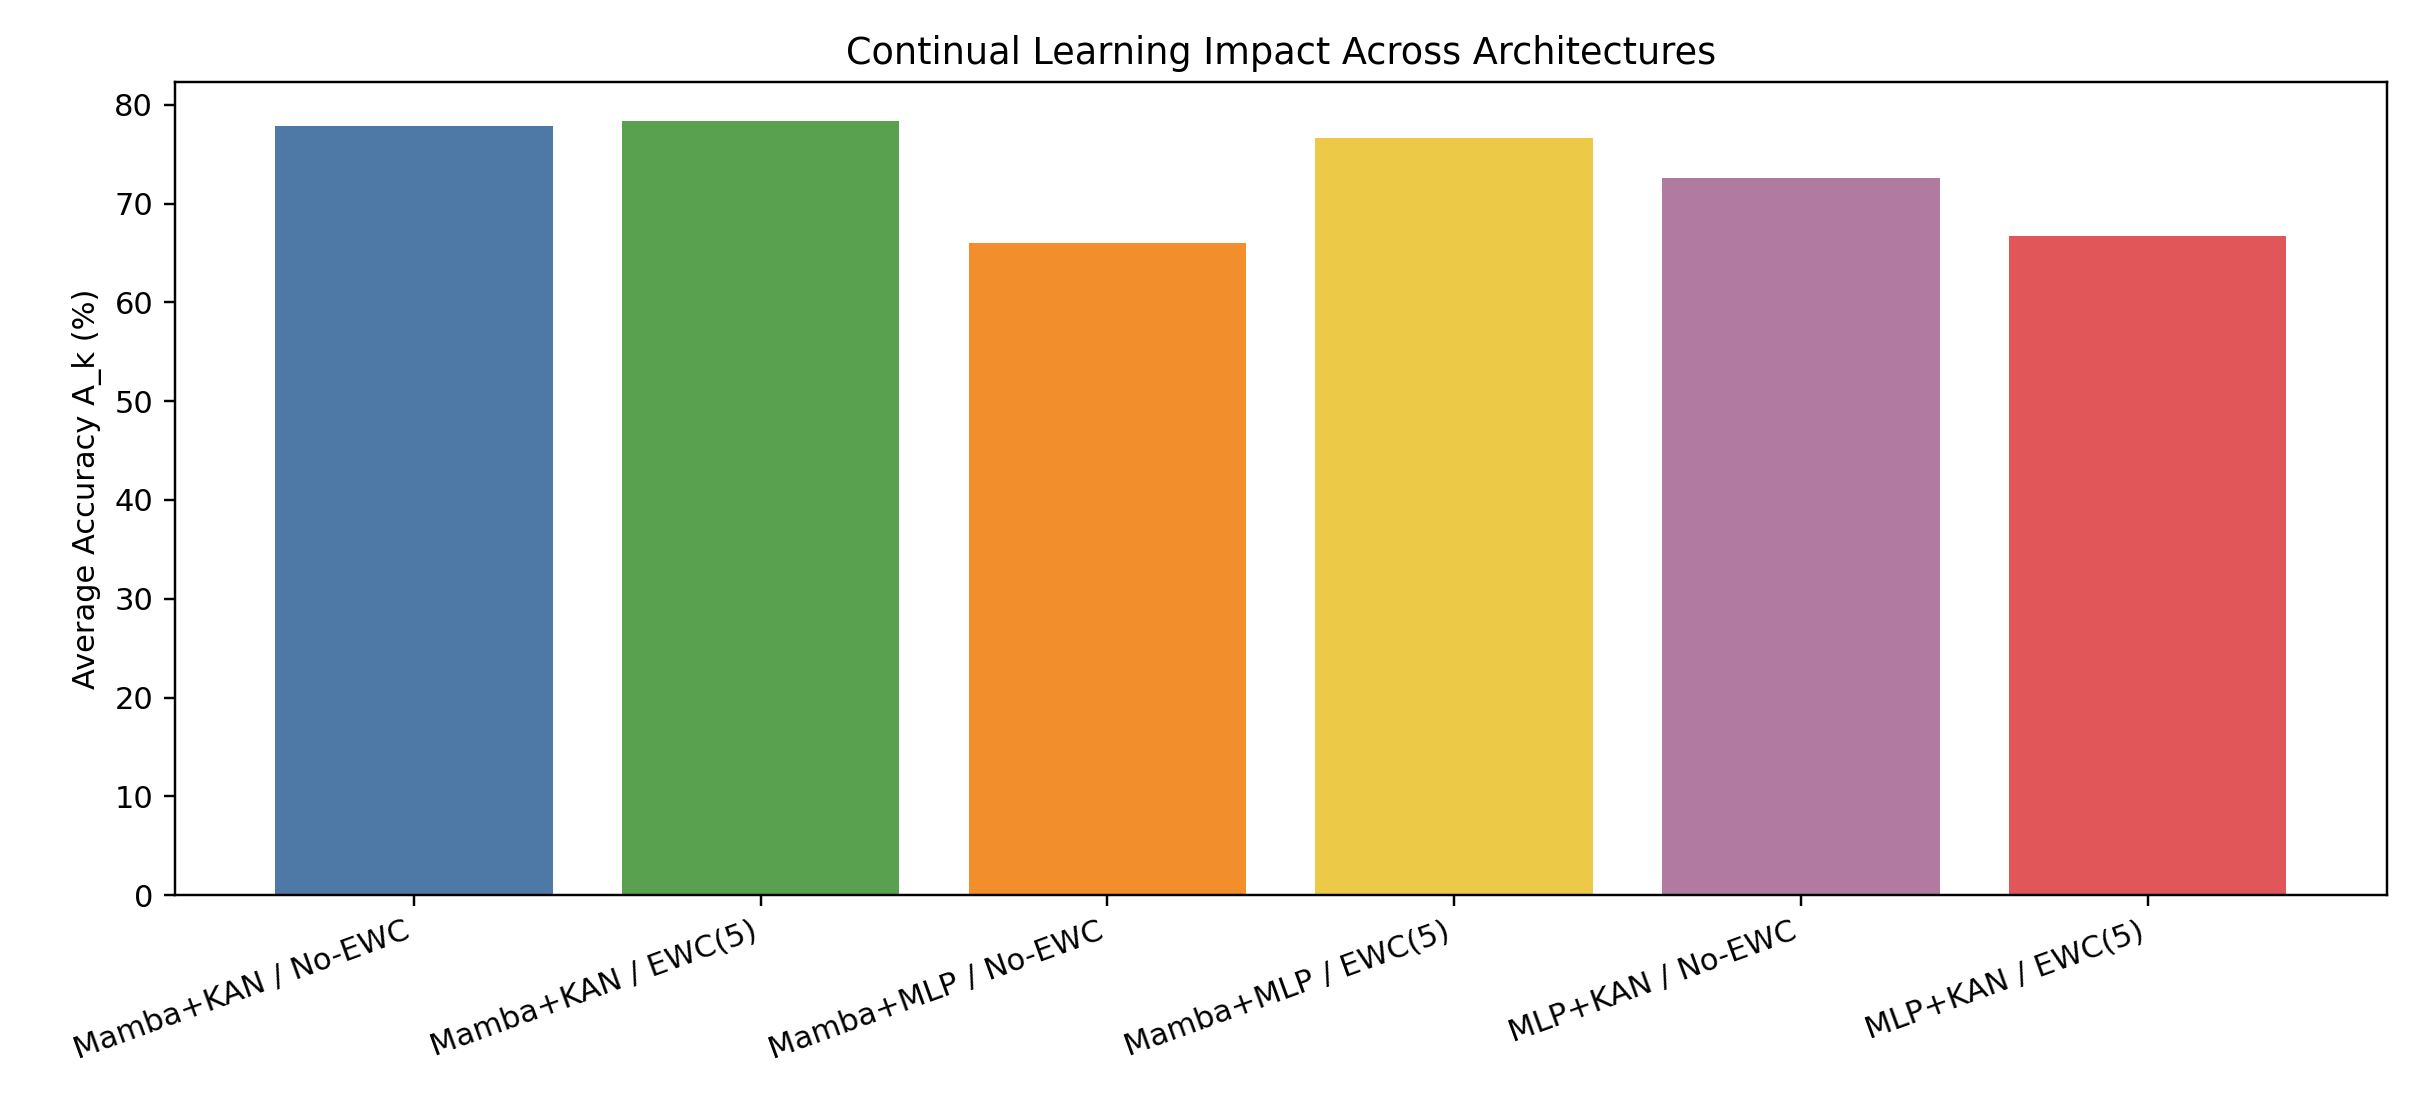
\includegraphics[width=0.48\textwidth]{figures/benchmark_ak_arch_cl.png}}
\caption{$A_k$ across architecture and continual-learning settings.}
\label{fig:ak}
\end{figure}
Figure~\ref{fig:ak} indicates the best average two-task performance for Mamba+KAN+EWC(5). This reflects improved stability-plasticity balance rather than pure adaptation gain.

\begin{figure}[htbp]
\centerline{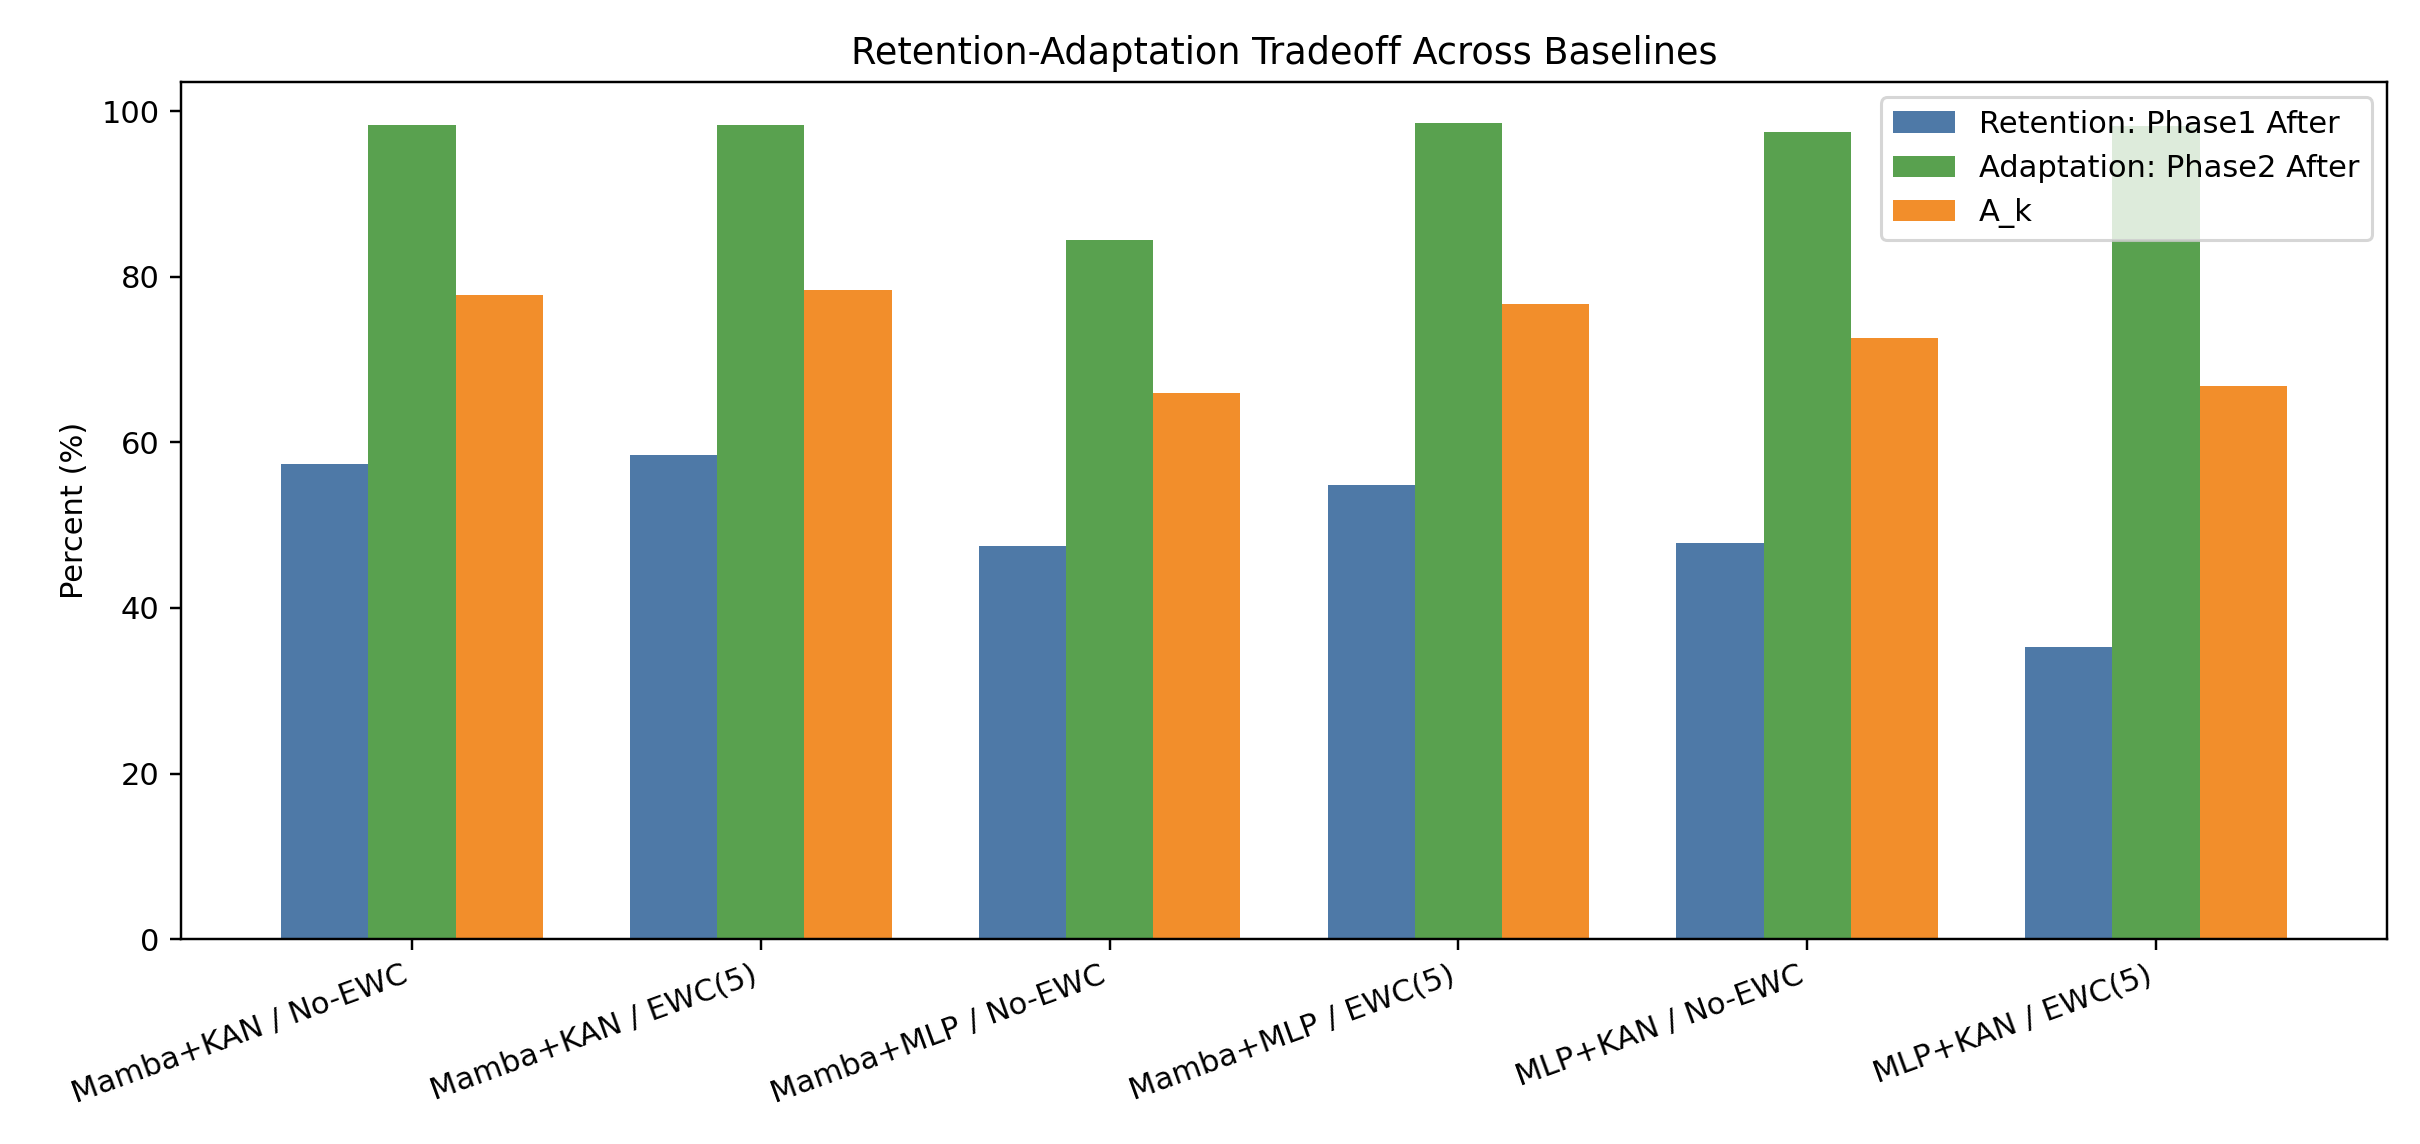
\includegraphics[width=0.48\textwidth]{figures/benchmark_retention_adaptation.png}}
\caption{Retention-adaptation tradeoff (Phase-1-after, Phase-2-after, and $A_k$).}
\label{fig:tradeoff}
\end{figure}
Figure~\ref{fig:tradeoff} shows that high Phase-2 accuracy alone is insufficient; retention can still collapse. The selected best setting is the one that keeps both metrics high simultaneously.

\begin{figure}[htbp]
\centerline{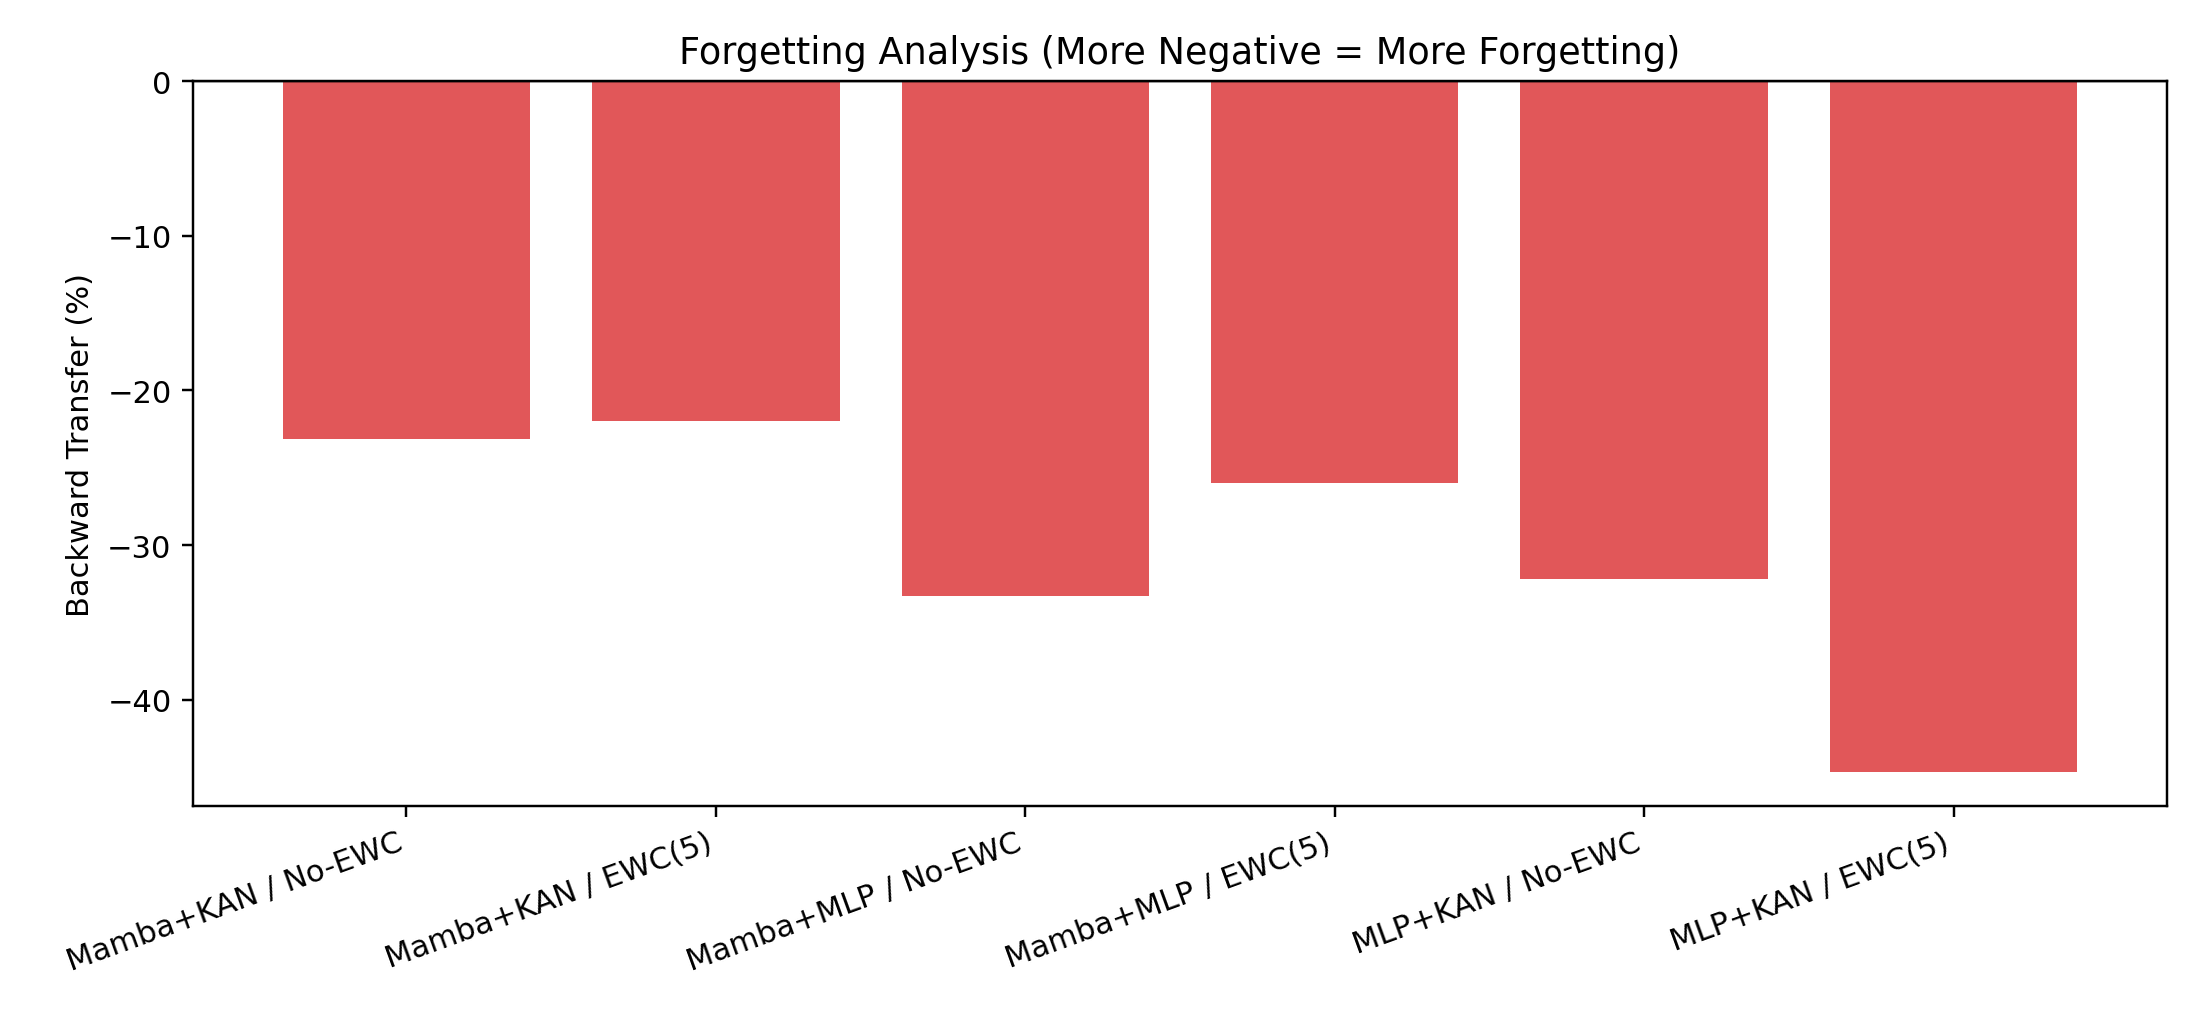
\includegraphics[width=0.48\textwidth]{figures/benchmark_bwt.png}}
\caption{Backward Transfer comparison (higher is better).}
\label{fig:bwt}
\end{figure}
Figure~\ref{fig:bwt} confirms forgetting across all settings (negative BWT), with relatively lower forgetting for Mamba+KAN+EWC(5).

\begin{figure}[htbp]
\centerline{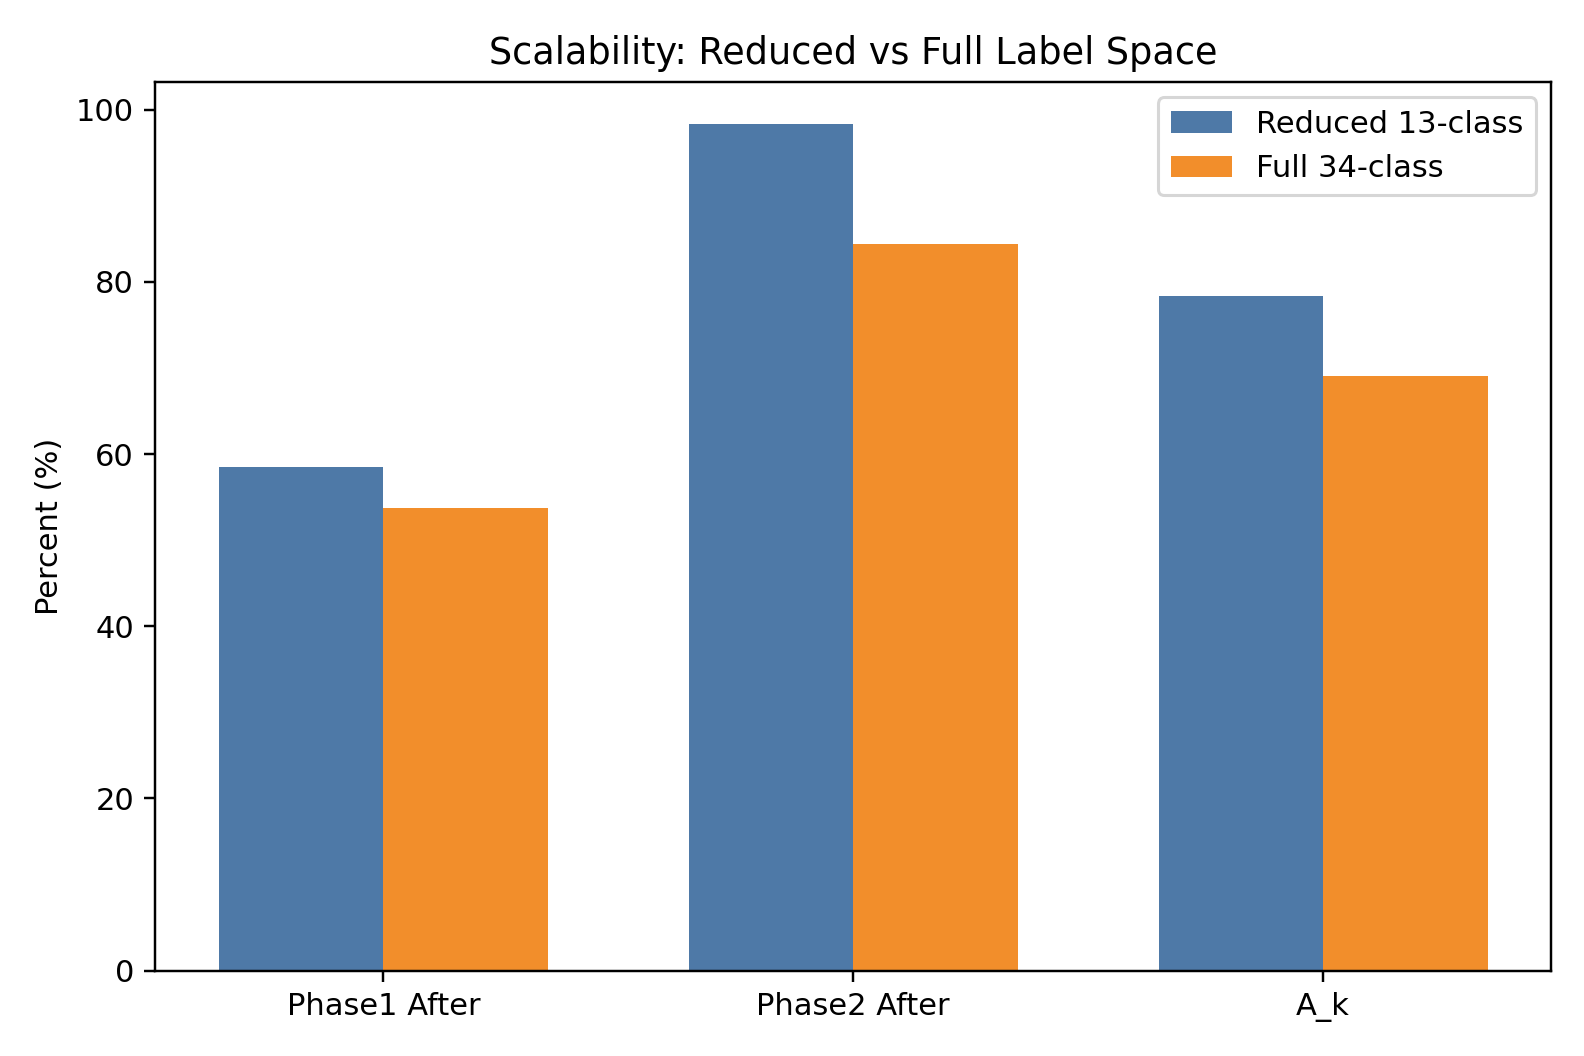
\includegraphics[width=0.48\textwidth]{figures/benchmark_reduced_vs_full.png}}
\caption{Reduced-label versus full 34-class benchmark.}
\label{fig:full}
\end{figure}
Figure~\ref{fig:full} quantifies the scalability gap: reduced protocols can overestimate deployment readiness.

\begin{figure}[htbp]
\centerline{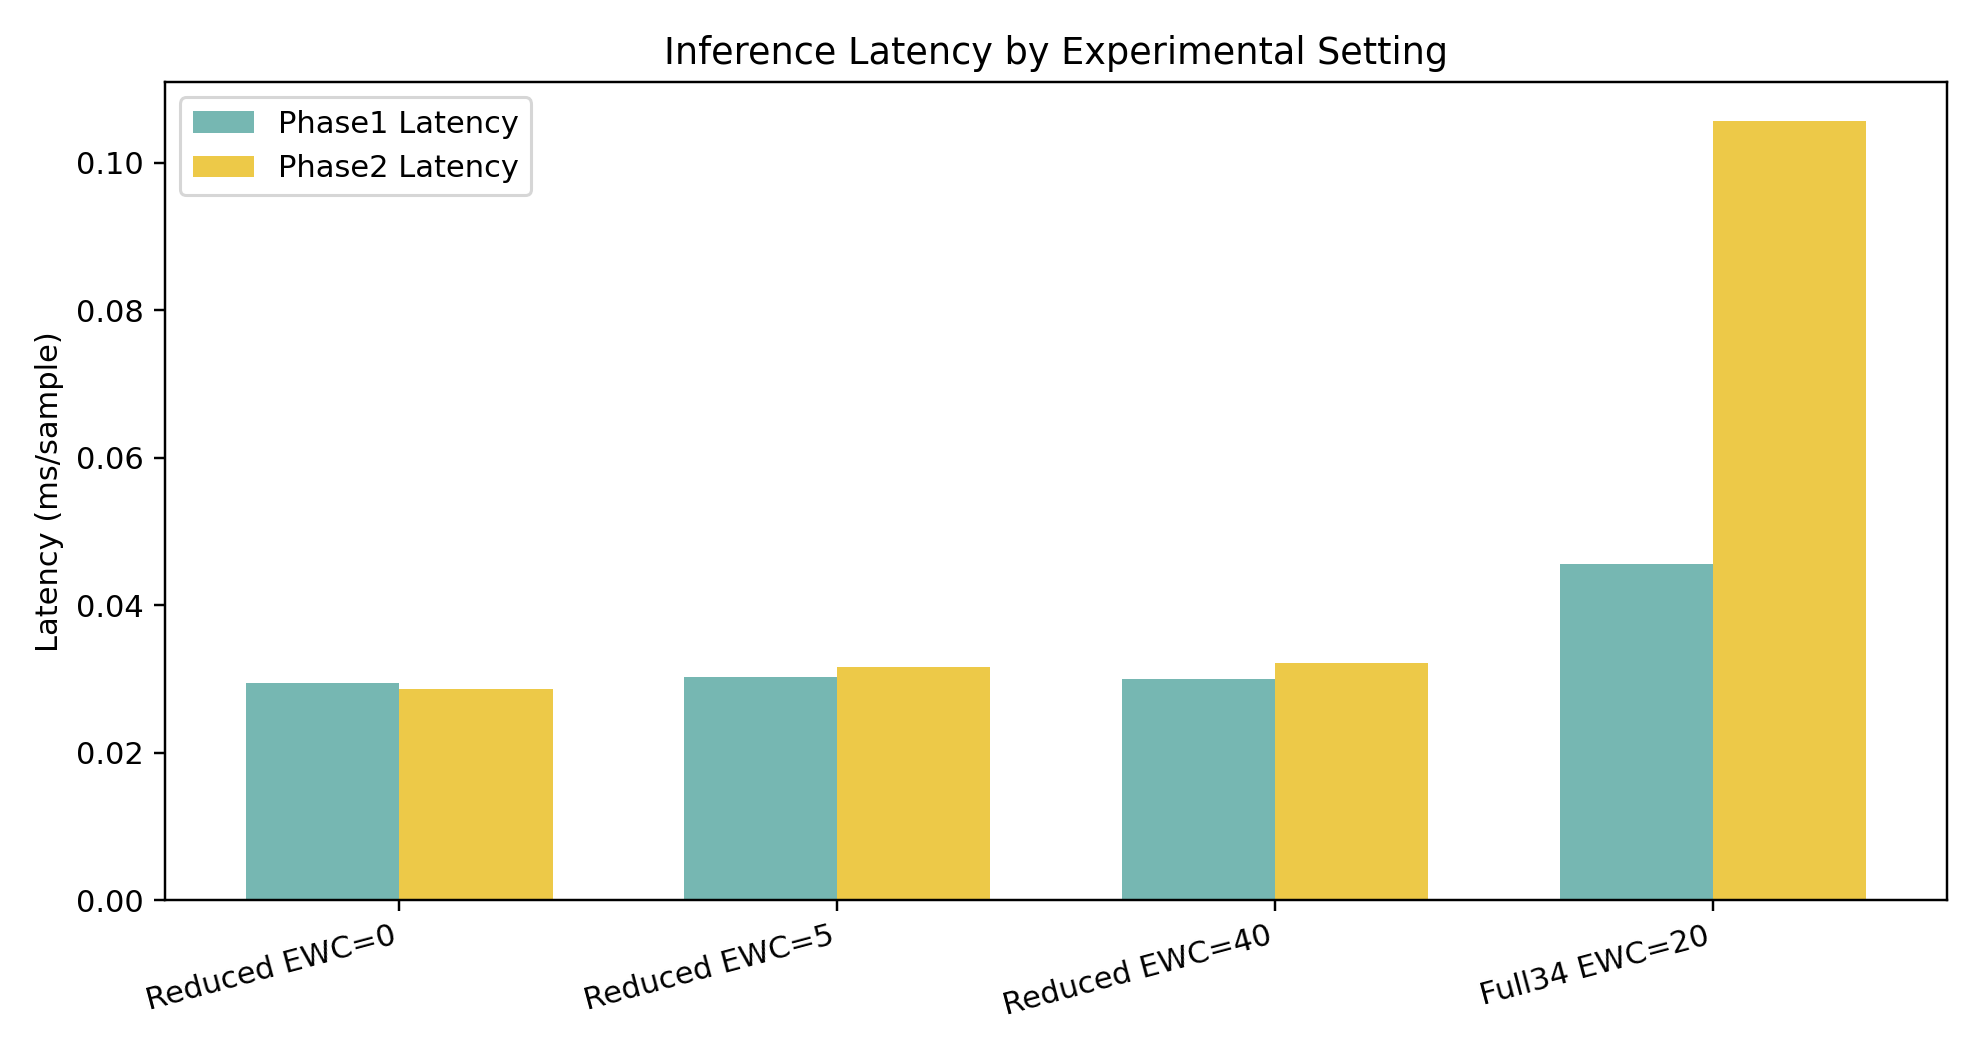
\includegraphics[width=0.48\textwidth]{figures/latency.png}}
\caption{Inference latency across settings (ms/sample).}
\label{fig:latency}
\end{figure}
Figure~\ref{fig:latency} shows sub-millisecond inference in all cases, indicating computational feasibility on resource-constrained hardware.

\begin{figure}[htbp]
\centerline{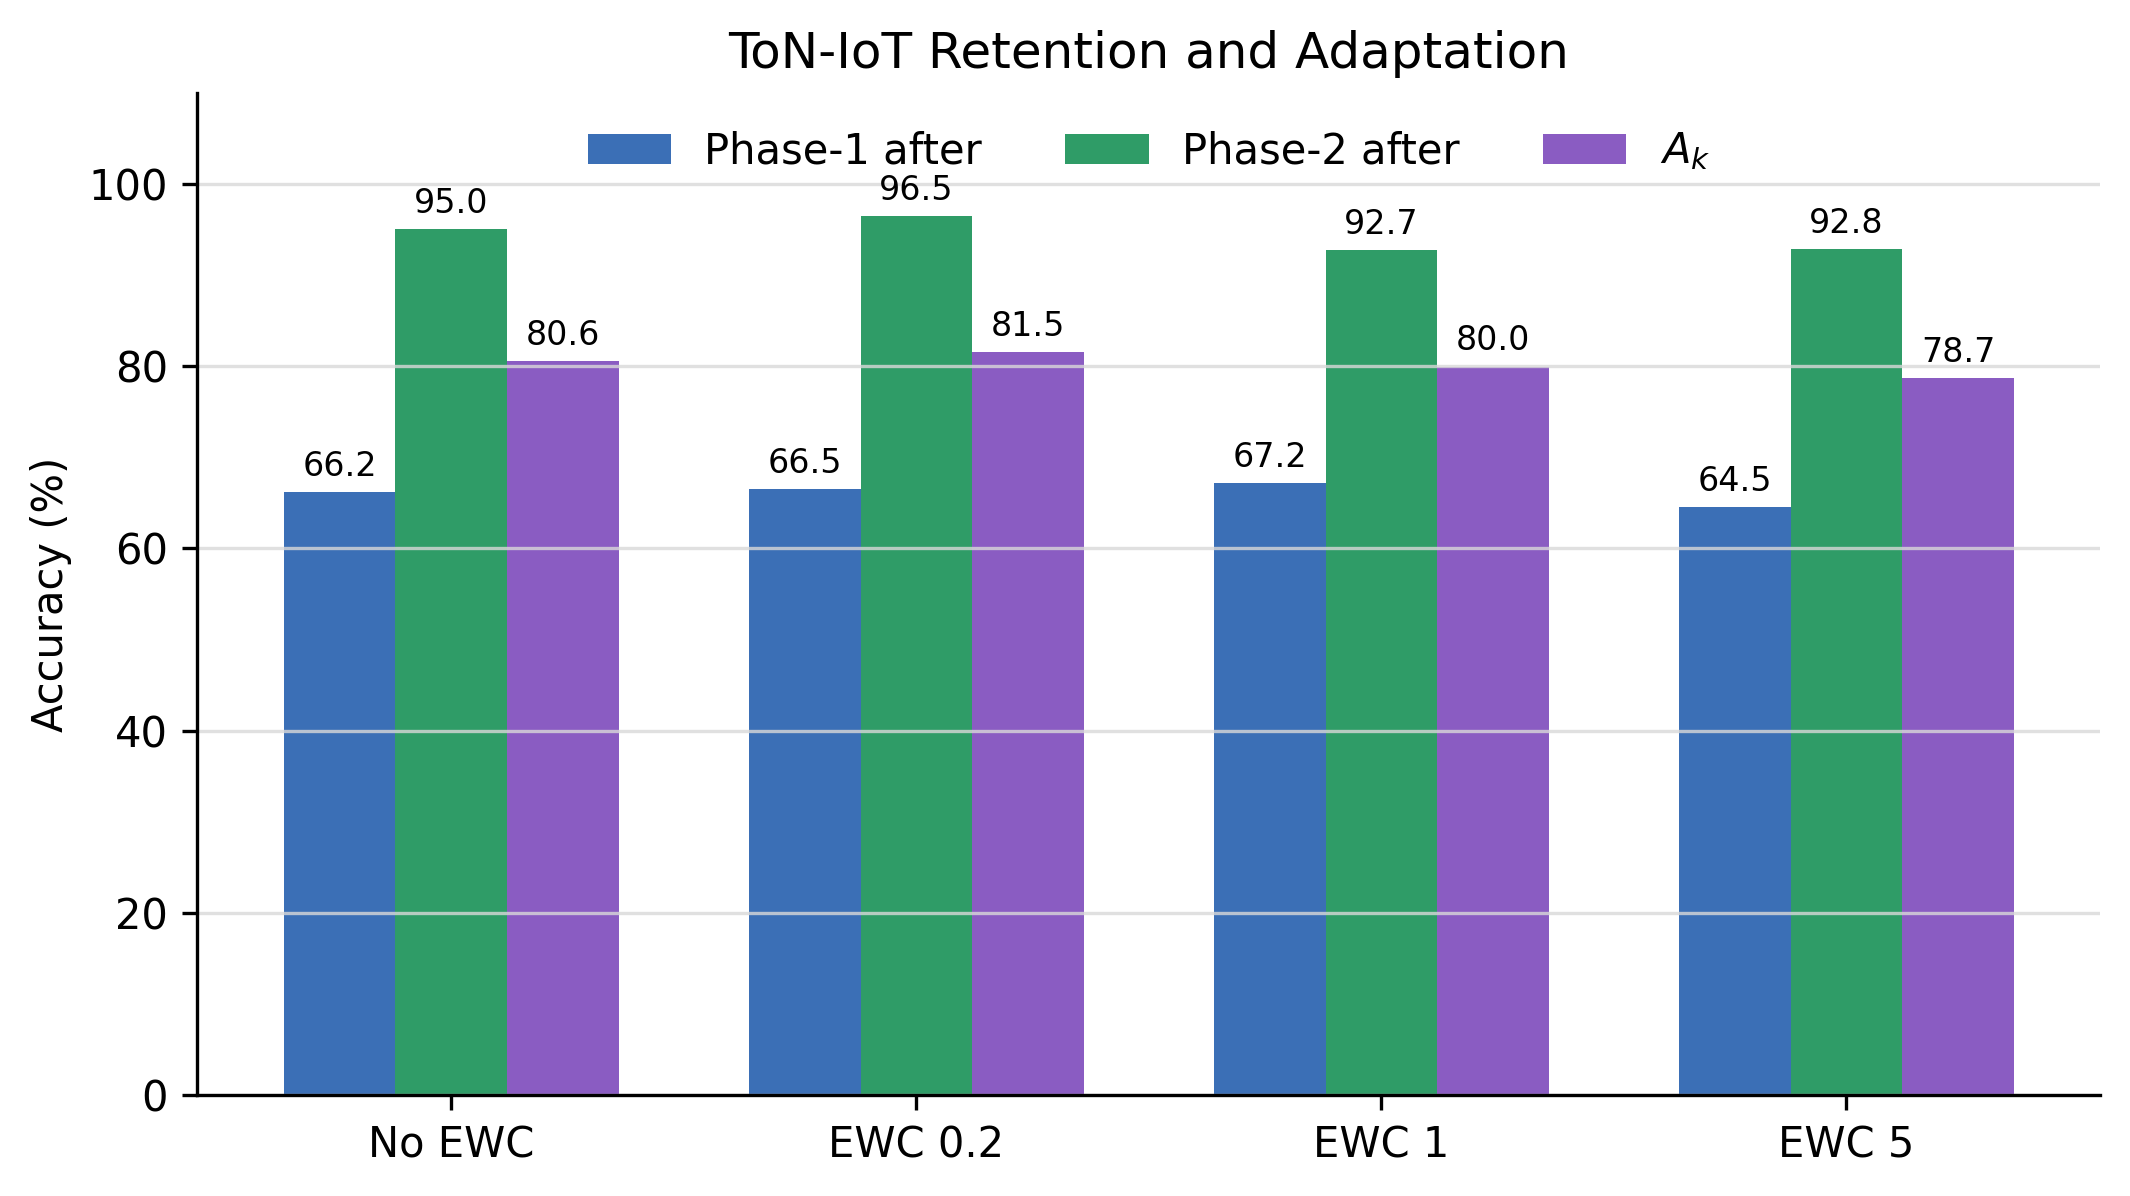
\includegraphics[width=0.48\textwidth]{figures/toniot_retention_adaptation.png}}
\caption{ToN-IoT retention-adaptation tradeoff across EWC strengths.}
\label{fig:toniot_tradeoff}
\end{figure}
Figure~\ref{fig:toniot_tradeoff} shows that the external dataset follows the same continual-learning pattern: high adaptation can coexist with substantial forgetting, so $A_k$ must be interpreted jointly with Phase-1-after and Phase-2-after accuracy.

\begin{figure}[htbp]
\centerline{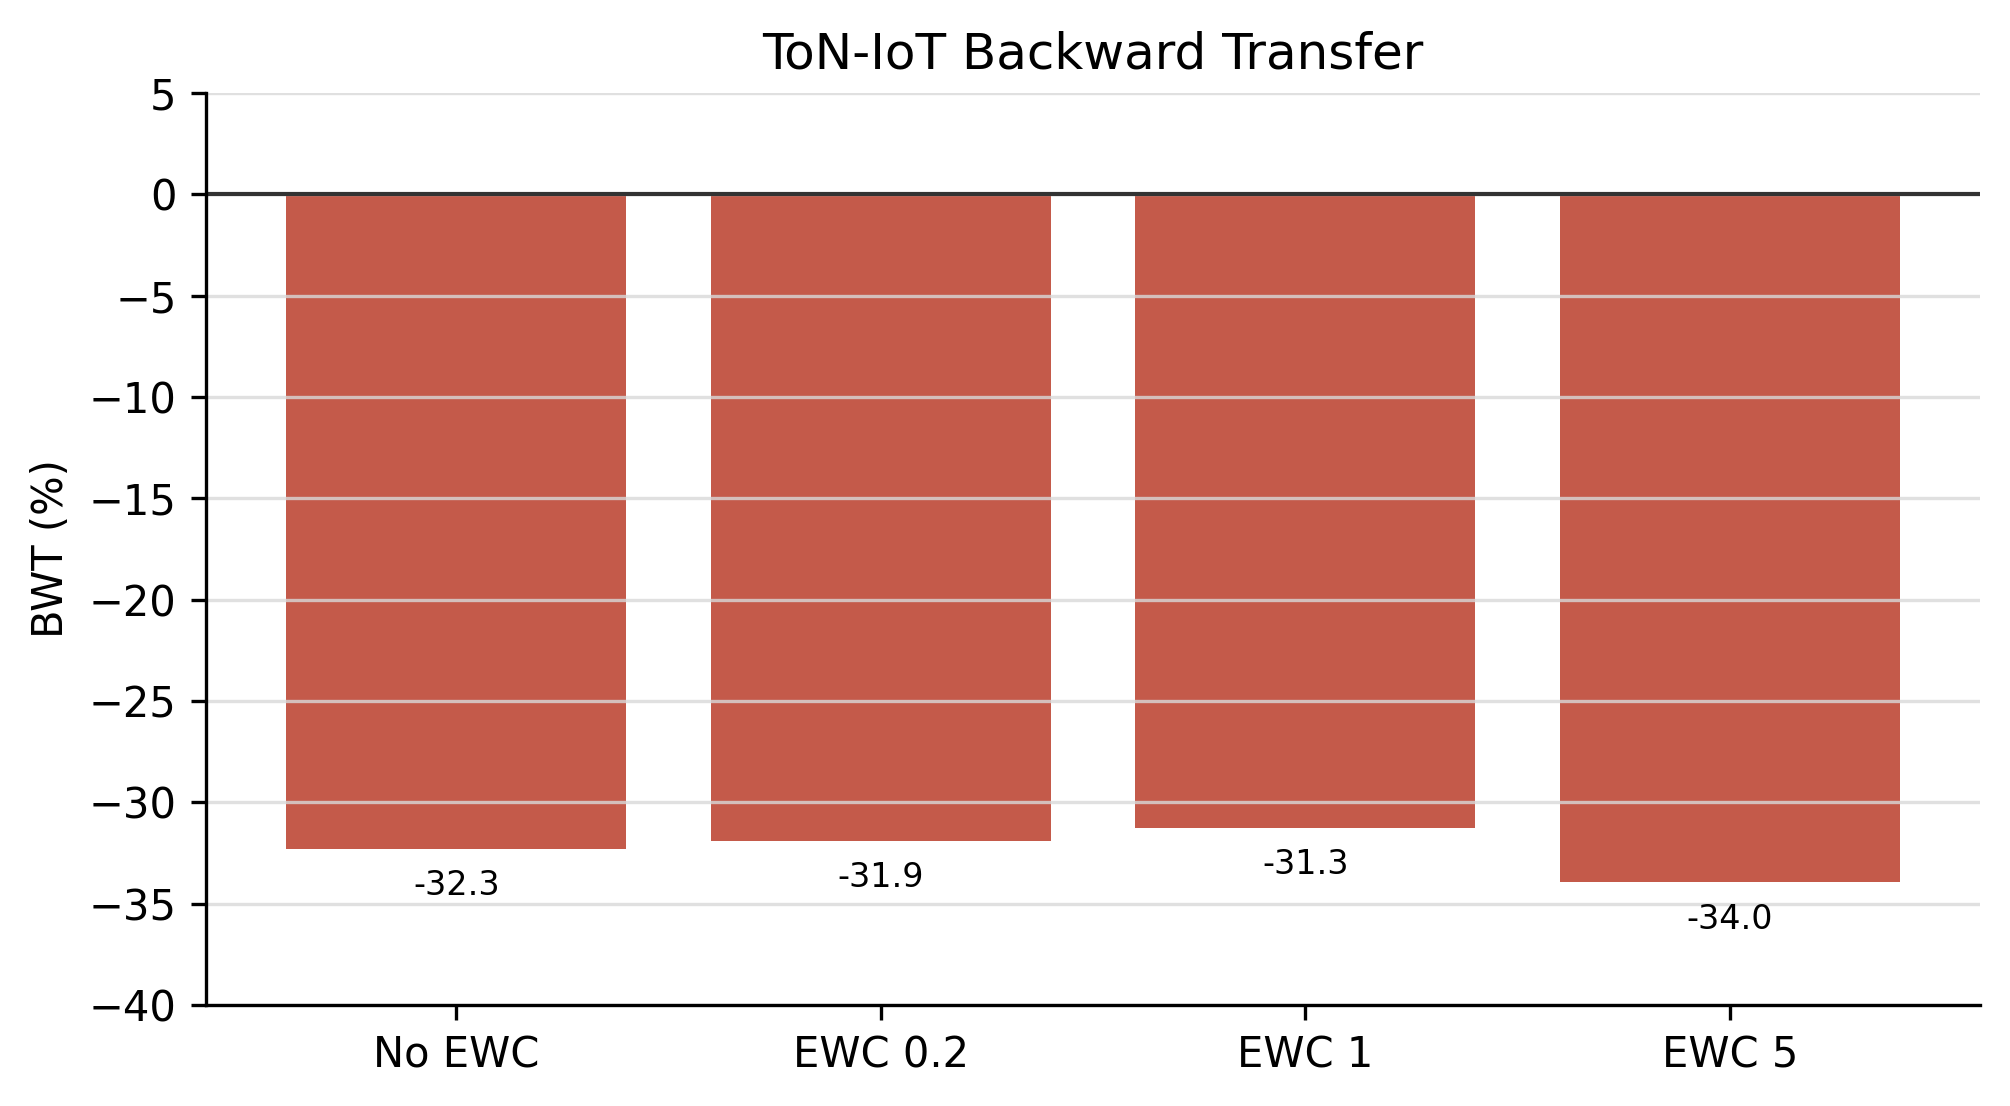
\includegraphics[width=0.48\textwidth]{figures/toniot_bwt.png}}
\caption{ToN-IoT Backward Transfer comparison (higher is better).}
\label{fig:toniot_bwt}
\end{figure}
Figure~\ref{fig:toniot_bwt} confirms that ToN-IoT also exhibits negative BWT. Light-to-moderate EWC reduces forgetting relative to direct sequential finetuning, while stronger EWC does not guarantee a better overall tradeoff.

\begin{figure}[htbp]
\centerline{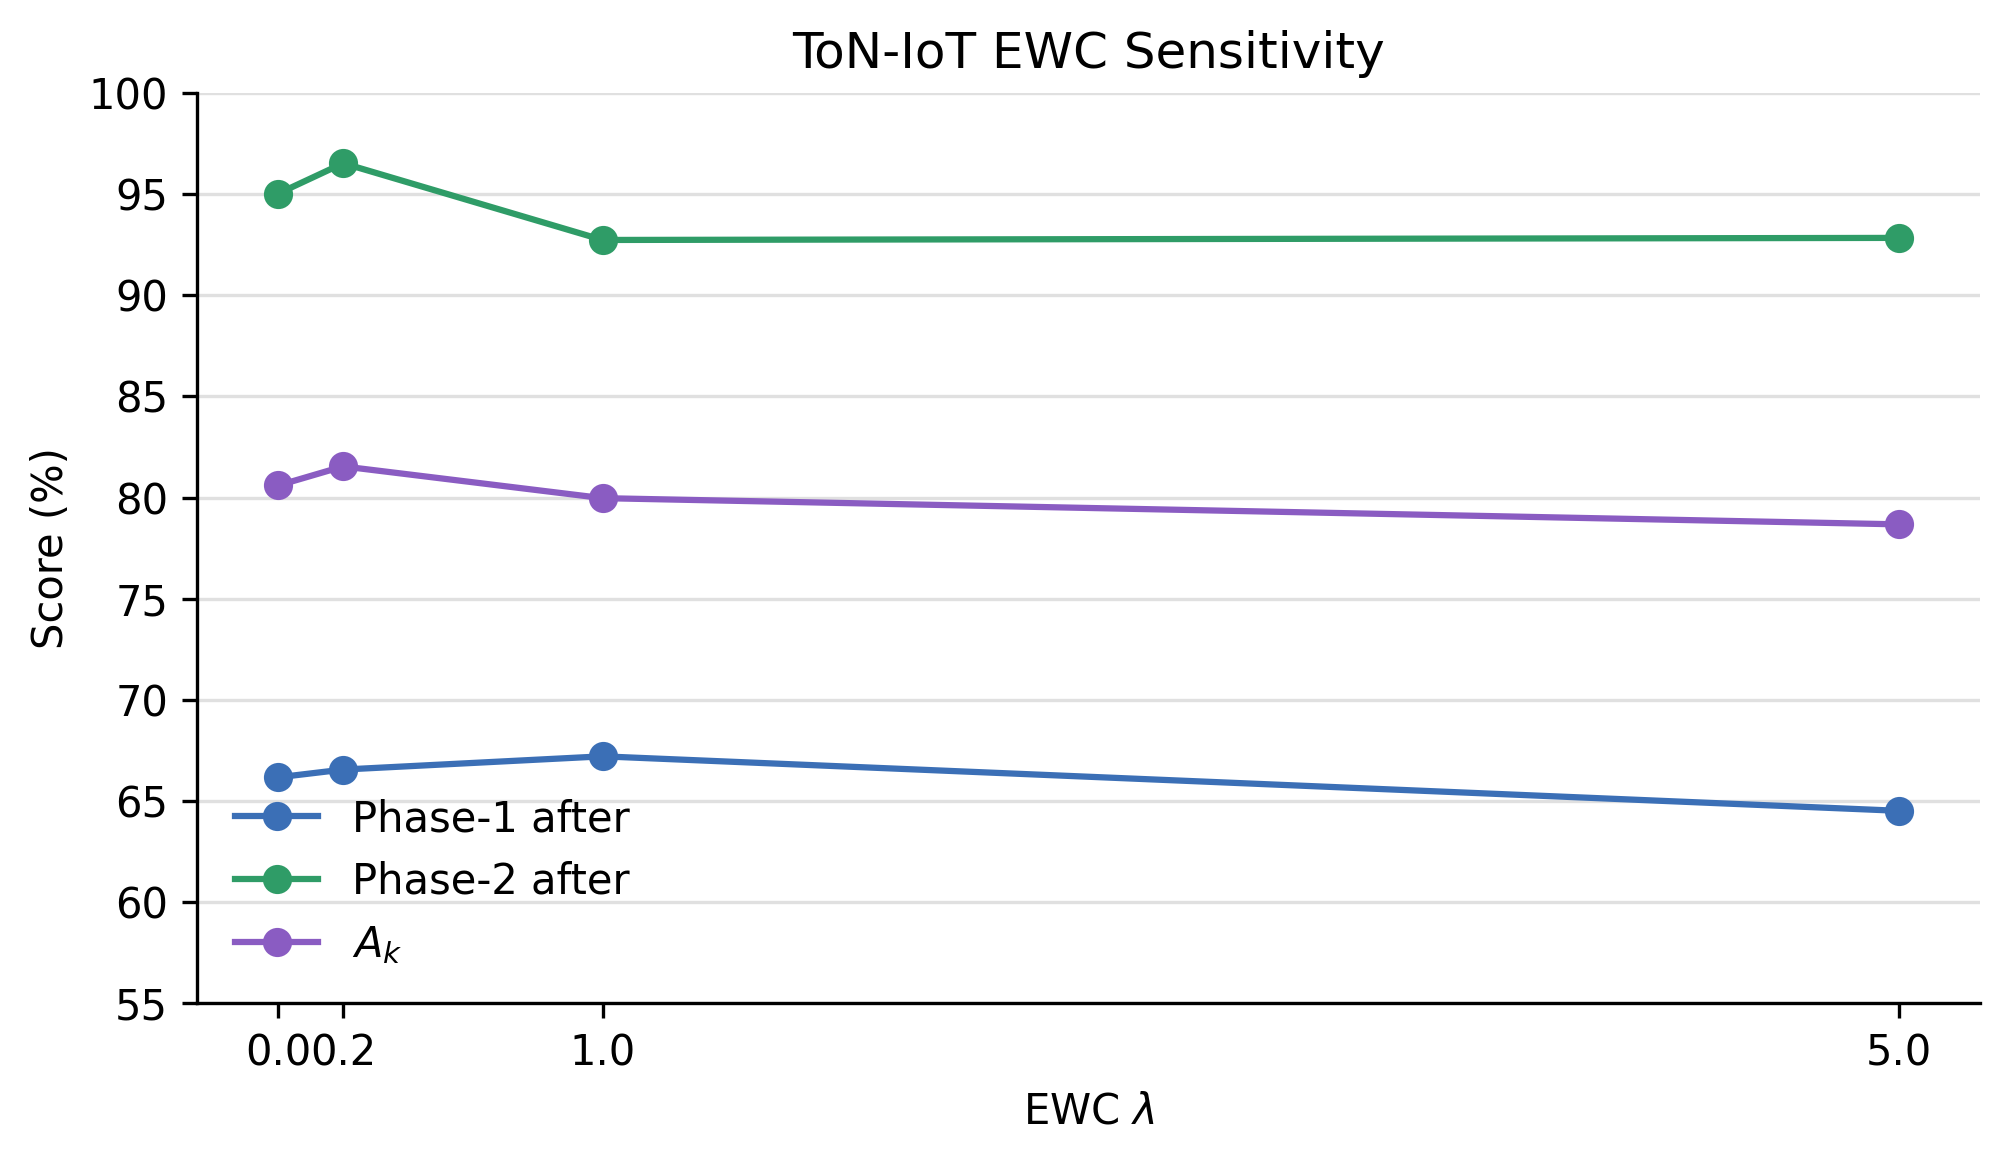
\includegraphics[width=0.48\textwidth]{figures/toniot_ewc_sweep.png}}
\caption{ToN-IoT EWC sensitivity for Phase-1 retention, Phase-2 adaptation, and $A_k$.}
\label{fig:toniot_sweep}
\end{figure}
Figure~\ref{fig:toniot_sweep} highlights the dataset-specific nature of EWC tuning. The best average accuracy occurs at $\lambda=0.2$, whereas larger values protect old-task behavior at the cost of new-task adaptation.

\begin{figure}[htbp]
\centerline{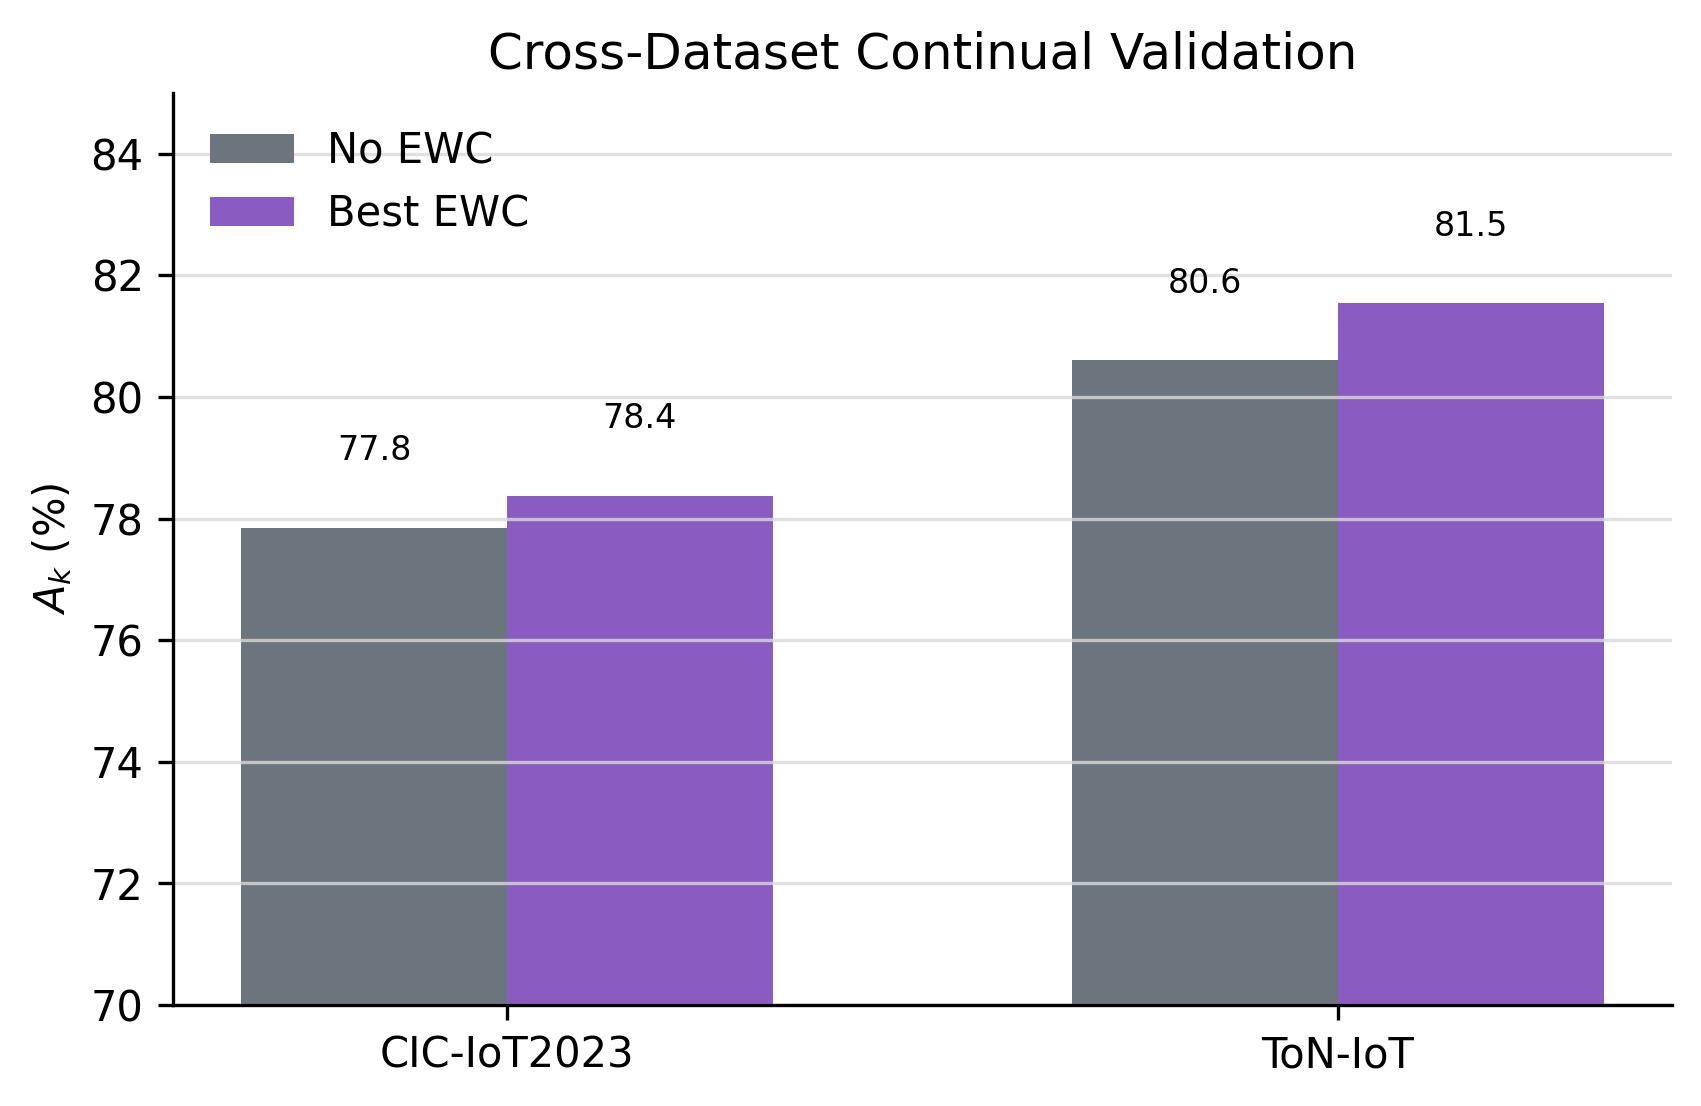
\includegraphics[width=0.48\textwidth]{figures/cross_dataset_validation.png}}
\caption{Cross-dataset comparison of Mamba+KAN with and without tuned EWC.}
\label{fig:cross_dataset}
\end{figure}
Figure~\ref{fig:cross_dataset} compares the main Mamba+KAN setting across CIC-IoT2023 and ToN-IoT. In both datasets, tuned EWC improves $A_k$ over no-EWC sequential finetuning, showing the same retention-adaptation pattern under a second label space.

\subsection{Extended Multi-Task Framework Validation}
To address the limitation that two phases are insufficient for a mature continual-learning benchmark, the codebase was refactored to support arbitrary task streams, LwF, ER, ER-ACE-style replay, DER++-style replay, EWC combinations, class-frequency-aware Fisher weighting, joint-training upper bounds, per-epoch histories, Fisher summaries, and multi-seed mean/std summaries. Table~\ref{tab:smoke4task} reports a deliberately small 4-task CIC-IoT2023 smoke run. These numbers are not used as publication-scale evidence because each task uses only 3000 training samples and one epoch; they verify that the extended protocol, metric computation, replay buffer, and figure pipeline execute correctly.

\begin{table}[htbp]
\caption{4-Task CIC-IoT2023 Smoke Validation of Extended Framework (Scores in \%)}
\label{tab:smoke4task}
\centering
\begin{tabular}{lcccc}
\toprule
Run & Seeds & $A_k$ & BWT & Forget. \\
\midrule
ER+EWC & 1 & 83.90 & 7.33 & 1.07 \\
DER++ + EWC & 1 & 85.00 & 8.33 & 0.30 \\
ER-ACE+EWC & 1 & 83.90 & 7.33 & 1.07 \\
Joint upper & 1 & 85.68 & -- & -- \\
ER+EWC & 2 & $82.40\pm2.12$ & $5.65\pm2.38$ & $2.68\pm2.29$ \\
\bottomrule
\end{tabular}
\end{table}

\begin{figure}[htbp]
\centerline{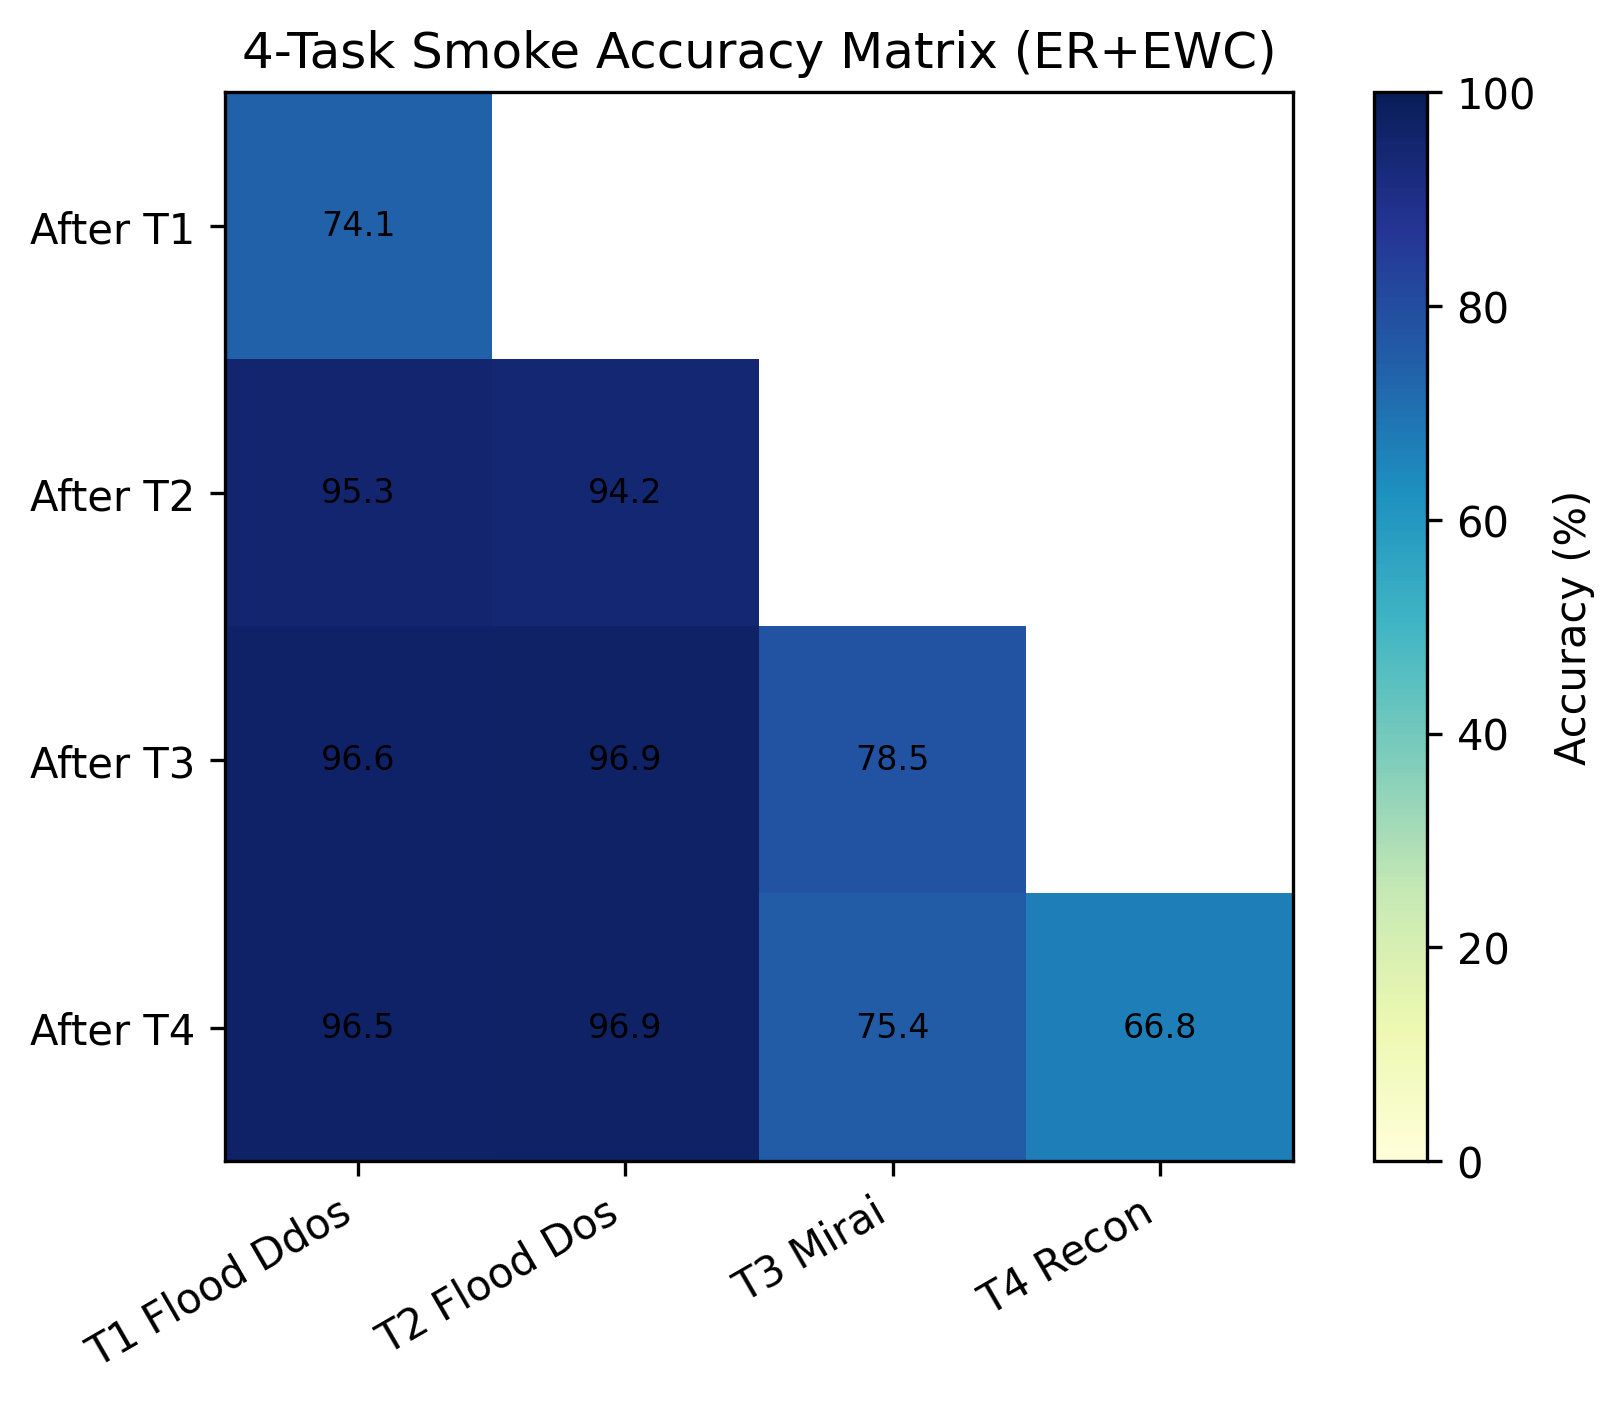
\includegraphics[width=0.48\textwidth]{figures/multitask_smoke_accuracy_matrix.png}}
\caption{Accuracy matrix for the 4-task ER+EWC smoke validation. Blank entries correspond to future tasks not yet seen at that training point.}
\label{fig:multitask_matrix}
\end{figure}

\begin{figure}[htbp]
\centerline{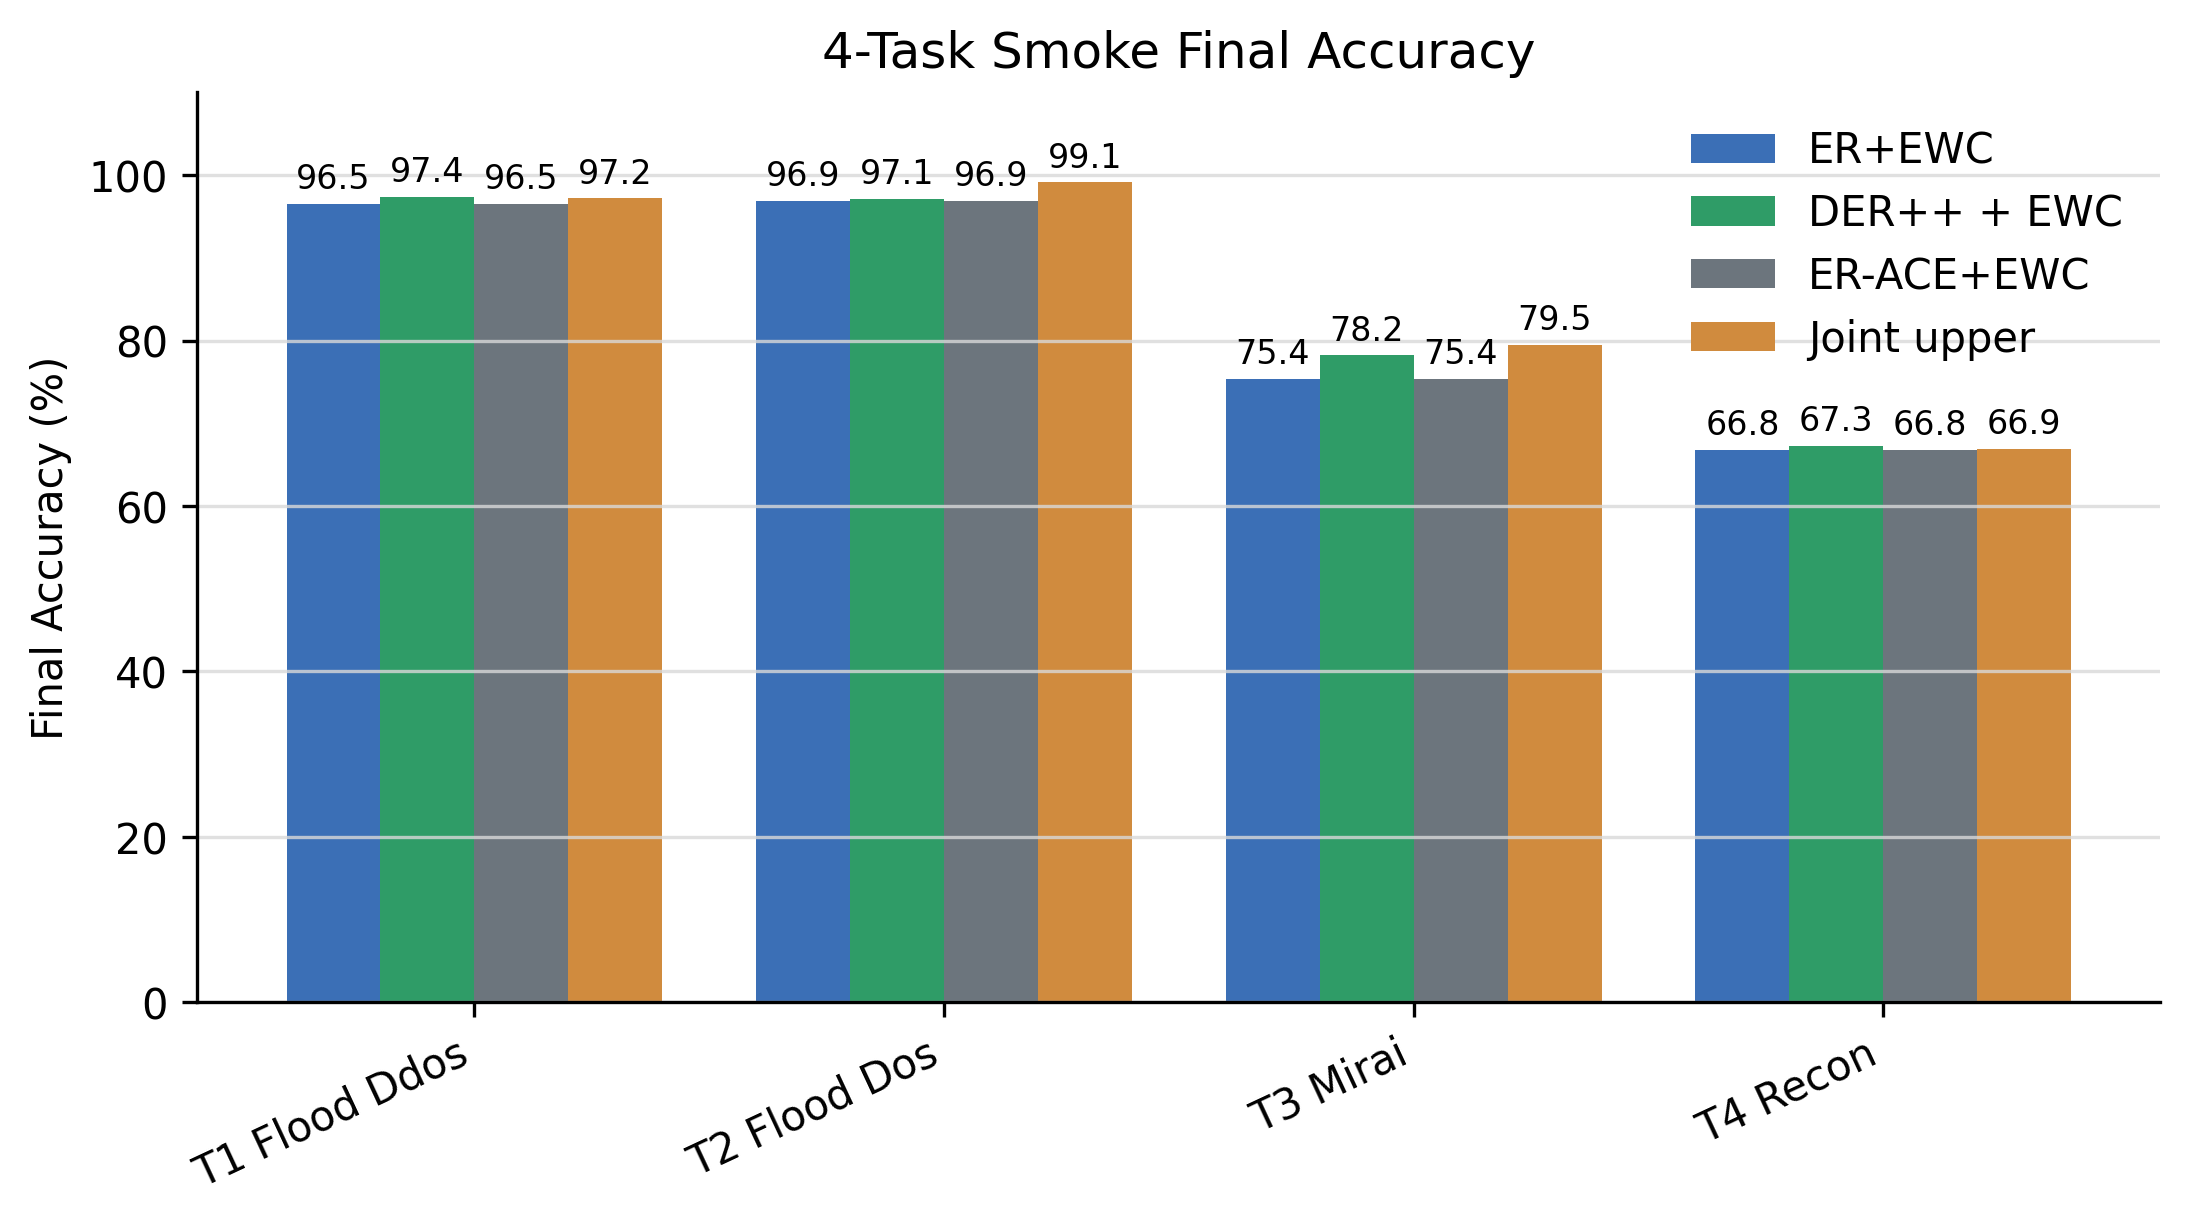
\includegraphics[width=0.48\textwidth]{figures/multitask_smoke_final_accuracy.png}}
\caption{Final per-task smoke accuracy for ER+EWC, ER-ACE+EWC, DER++ + EWC, and the joint-training upper-bound runner. The run validates stronger-baseline code paths, not final benchmark performance.}
\label{fig:multitask_final}
\end{figure}

\begin{figure}[htbp]
\centerline{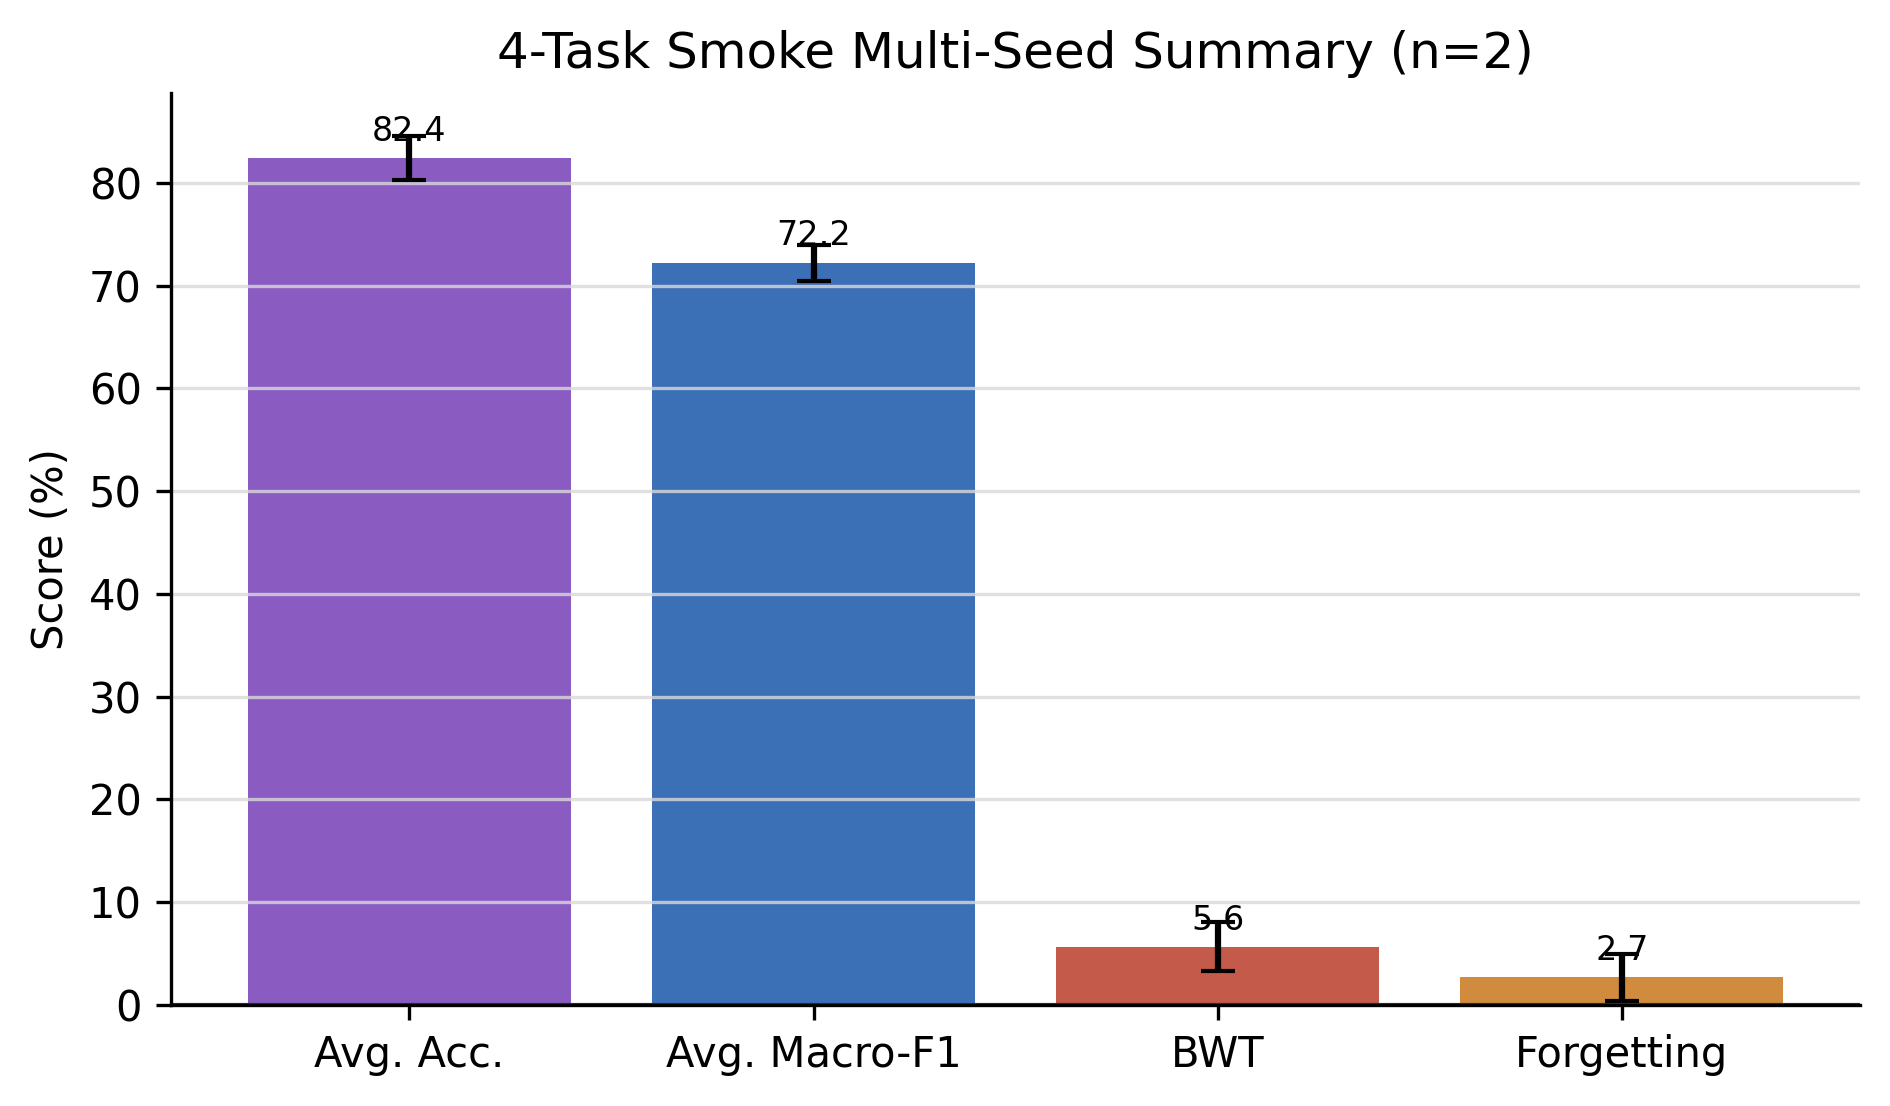
\includegraphics[width=0.48\textwidth]{figures/multiseed_smoke_summary.png}}
\caption{Two-seed smoke summary for ER+EWC showing that the benchmark runner exports mean and standard deviation metrics.}
\label{fig:multiseed_summary}
\end{figure}

\section{Discussion}
\subsection{Scope of the Claim}
The results should be interpreted as a security-oriented evaluation study, not as evidence of a new state-of-the-art IDS architecture. Mamba--KAN style IDS modeling already exists in static settings, and EWC is a standard regularization-based continual-learning method. The contribution here is the controlled measurement of sequential IDS updates, the identification of protocol choices that materially change whether retention is validly measured, the comparison against related architectural variants, and an implementation path toward longer task streams with replay baselines.

\subsection{Protocol Validity and Stabilization}
The active-class mask is central to the task-incremental formulation. When the classifier is trained over a union label space but only a subset of classes is valid in the current phase, unconstrained softmax training allows inactive classes to absorb probability mass even though they are not valid task labels. This creates degenerate predictions and makes retention/adaptation metrics difficult to interpret. Restricting the loss and prediction rule to $\mathcal{C}_k$ makes the protocol internally consistent. Bounded inverse-frequency class weighting is also required because extreme rare-class weights can destabilize the small two-phase setting.

\subsection{Cross-Dataset Interpretation}
The ToN-IoT validation is best read as an external replication of the same qualitative pattern rather than a complete generalization claim. The absolute numbers differ because the label space, feature semantics, and class imbalance differ, especially the rare mitm class in ToN-IoT. However, the qualitative behavior is consistent: sequential training adapts to new classes but forgets prior ones, and tuned EWC improves the average retention-adaptation balance. The best EWC coefficient is lower on ToN-IoT than on CIC-IoT2023, which reinforces that regularization strength should be treated as a protocol hyperparameter rather than a universal constant.

\subsection{How to State the Improvement}
If asked whether this paper is better than the MAMBA--KAN reference, the precise answer is: on CIC-IDS2017, the local Mamba+KAN implementation achieves higher weighted/global F1 (97.92\%) than the reference paper's reported CICIDS2017 F1 (96.54\%), giving a direct same-dataset numerical improvement of 1.38 percentage points. However, because the reference paper does not specify the multiclass averaging convention, and because our macro-F1 is 69.44\% due to extremely rare classes, this should be stated as a weighted/static improvement rather than a universal static state-of-the-art claim. Separately, the continual-learning result is a protocol and retention analysis: adding tuned EWC to Mamba+KAN improves $A_k$ from 77.84\% to 78.38\%, improves BWT from $-23.11$ to $-21.99$, and improves Phase-1-after-Phase-2 retention from 57.34\% to 58.46\% in the original single-seed pair, but a three-seed rerun does not confirm that EWC(5) is reliably better than no-EWC. The same retention-adaptation pattern is externally validated on ToN-IoT, where tuned EWC improves $A_k$ from 80.60\% to 81.54\%.

\subsection{Threats to Deployment}
For a production IDS, negative BWT is not an abstract continual-learning score; it means that an update for new attack families can silently reduce detection quality for attacks the SOC already believed were covered. In the best single-seed CIC-IoT2023 EWC point estimate, BWT $=-21.99$ corresponds to a 21.99 percentage-point drop in Phase-1 task accuracy after learning Phase 2. Under the Phase-1 test distribution, this is the difference between 80.45\% and 58.46\% correct classification for previously learned benign/flooding traffic. If a deployment window contained 100,000 Phase-1-like events after the update, the same drop would correspond to roughly 21,990 additional misclassified events relative to the pre-update model. Because the benchmark is multi-class and includes benign rows, this number should not be read as an exact false-negative count; operationally, it is a warning that post-update validation must include old attack families, not only the newly added threat phase.

The joint-training upper bound clarifies the deployment gap. A model retrained from scratch on both reduced-protocol phases reaches $A_k=89.79\%$, whereas the best sequential point estimate reaches $A_k=78.38\%$ and the three-seed sequential means are lower. In operational terms, compact regularization-only updates are attractive because they avoid full retraining cost, but the present evidence does not justify deploying them without replay, recalibration, or rollback monitoring. A practical IDS pipeline should track old-family recall after every update, enforce active-task assumptions explicitly if the deployment is task-incremental, and trigger full retraining or stronger replay when retention falls below the SOC's tolerated missed-alert budget.

\subsection{Why EWC Hurts MLP+KAN}
The MLP+KAN result is a useful negative case rather than noise to hide. Relative to MLP+KAN without EWC, EWC reduces Phase-1-after accuracy by 12.44 points and $A_k$ by 5.86 points while improving Phase-2 accuracy by only 0.72 points. This suggests that the Fisher penalty constrains parameters that the shallow feed-forward backbone needs to repurpose for old-task retention, while the KAN head still adapts to the new phase. A fuller explanation requires Fisher-overlap and parameter-drift analysis, which the updated code now records for future full-scale runs.

\subsection{Threats to Validity}
\begin{itemize}
\item The main full-scale benchmark uses two phases, which is the minimum possible continual-learning setting. The new 4-task run is a smoke validation only; it verifies that the framework executes but cannot serve as journal-grade evidence for multi-task continual learning.
\item The implemented LwF, ER-ACE, and DER++ baselines are not yet reported at full scale on four- or five-task streams. A mature journal submission should include those runs, preferably with a joint upper bound and identical task construction.
\item The two main reduced Mamba+KAN settings now include three-seed summaries, but the remaining architecture variants, ToN-IoT sweep, full34 run, and stronger-baseline paths are still point estimates on one hardware stack. Multi-seed results across all architecture variants are needed before making a robust algorithmic ranking claim.
\item Six epochs per phase may not fully characterize convergence; longer schedules and learning-rate warmup/cosine decay should be evaluated.
\item Parameter-isolation baselines are not yet implemented, and class-frequency-aware Fisher weighting is implemented but not yet evaluated at publication scale.
\item The CIC-IDS2017 static comparison is matched by dataset but is not an exact reproduction of the reference paper's private preprocessing, training schedule, or F1 averaging convention, so it should be read as a strong same-dataset check rather than a guaranteed reproduction.
\item File-order split approximates temporal drift but is not a perfect chronological replay.
\item ToN-IoT was converted from one public CSV into stratified shards so that the existing file-split protocol could be reused.
\item Reduced protocol may under-represent full-scale operational complexity.
\item Phase-aware masking assumes the active task is known at evaluation time; open class-incremental detection is a harder setting.
\end{itemize}

\section{Future Work}
The following extensions are prioritized for stronger retention and publication-grade completeness:
\begin{enumerate}
\item Run the implemented LwF, ER, ER-ACE-style, DER++-style, class-frequency-aware Fisher, and joint-training upper-bound baselines at full scale on four- and five-task CIC-IoT2023 and ToN-IoT streams. This is the main missing experiment for a journal-grade continual-learning claim.
\item Add a parameter-isolation method such as PackNet.
\item Extend multi-seed mean, standard deviation, confidence intervals, and statistical significance tests to all architecture variants, ToN-IoT settings, stronger continual baselines, and full-label runs using the benchmark runner.
\item Add matched static IDS baselines to contextualize accuracy, macro-F1, and latency against non-continual training.
\item Increase epochs and adopt warmup plus cosine learning-rate scheduling, with convergence curves for all tasks.
\item Add a Fisher-overlap or parameter-drift analysis to explain when EWC protects useful representations and when it blocks adaptation.
\item Investigate an IDS-specific CL method combining small exemplar replay, active-class calibration, and superclass-aware retention metrics.
\end{enumerate}

\section{Conclusion}
This paper presents a reproducible continual-learning IDS benchmark with architectural and algorithmic ablations. The central finding is that protocol design materially affects whether continual IDS results are valid: active-class logit masking and bounded class weighting are necessary before retention, adaptation, and BWT can be interpreted in a task-incremental security setting. On CIC-IoT2023, moderate EWC with Mamba+KAN gives the best original reduced-protocol point estimate, but a new three-seed rerun shows that the EWC(5) gain is not robust under the current runner. The 12-epoch joint-training upper bound reaches $A_k=89.79\%$, making the sequential-update gap explicit, and the 34-class CIC-IoT2023 reference run reveals the remaining gap to robust full-label retention. On the independent ToN-IoT Network dataset, light EWC improves $A_k$ over no-EWC sequential finetuning, replicating the retention-adaptation pattern beyond a single dataset. A same-dataset static CIC-IDS2017 check strengthens the comparison with the MAMBA--KAN reference: the local Mamba+KAN model reaches 97.92\% weighted F1 versus the reference paper's reported 96.54\% CICIDS2017 F1, although macro-F1 remains 69.44\% because of rare attack classes. The codebase now supports longer task streams, LwF, replay baselines, joint-training upper bounds, class-frequency-aware Fisher weighting, Fisher summaries, and multi-seed summaries, and the included smoke validation confirms that this extended pipeline runs. Across the full reported continual datasets, negative BWT remains, so the method should be viewed as a protocol-validity contribution and measured baseline rather than a complete solution to catastrophic forgetting. These findings motivate full-scale LwF/ER/ER-ACE/DER++ runs, parameter-isolation baselines, statistical testing, rare-class calibration, and IDS-specific replay methods.

\begin{thebibliography}{00}
\bibitem{zhao2025}
Y. Zhao and H. Zhang, ``Research on a Network Traffic Intrusion Detection System Based on MAMBA-KAN,'' in \textit{Proc. CAIBDA}, 2025, doi:10.1109/CAIBDA65784.2025.11183131.

\bibitem{kirkpatrick2017}
J. Kirkpatrick \textit{et al.}, ``Overcoming catastrophic forgetting in neural networks,'' \textit{PNAS}, vol. 114, no. 13, pp. 3521--3526, 2017.

\bibitem{gu2023}
A. Gu and T. Dao, ``Mamba: Linear-time sequence modeling with selective state spaces,'' arXiv:2312.00752, 2023.

\bibitem{liu2024}
Z. Liu \textit{et al.}, ``KAN: Kolmogorov-Arnold Networks,'' arXiv:2404.19756, 2024.

\bibitem{zenke2017}
F. Zenke, B. Poole, and S. Ganguli, ``Continual Learning Through Synaptic Intelligence,'' in \textit{ICML}, 2017.

\bibitem{aljundi2018}
R. Aljundi \textit{et al.}, ``Memory Aware Synapses: Learning what (not) to forget,'' in \textit{ECCV}, 2018.

\bibitem{li2017}
Z. Li and D. Hoiem, ``Learning without Forgetting,'' \textit{IEEE TPAMI}, vol. 40, no. 12, pp. 2935--2947, 2018.

\bibitem{ciciot2023}
E. C. Pinto Neto, S. Dadkhah, R. Ferreira, A. Zohourian, R. Lu, and A. A. Ghorbani, ``CICIoT2023: A real-time dataset and benchmark for large-scale attacks in IoT environment,'' \textit{Sensors}, vol. 23, no. 13, art. no. 5941, 2023, doi:10.3390/s23135941.

\bibitem{toniot2020}
N. Moustafa, ``A new distributed architecture for evaluating AI-based security systems at the edge: Network TON\_IoT datasets,'' \textit{Sustainable Cities and Society}, vol. 72, art. no. 102994, 2021, doi:10.1016/j.scs.2021.102994.

\bibitem{li2025citadel}
E. Li, O. Gungor, Z. Shang, and T. Rosing, ``CITADEL: Continual Anomaly Detection for Enhanced Learning in IoT Intrusion Detection,'' arXiv:2508.19450, 2025.

\bibitem{zhang2025ssf}
X. Zhang, R. Zhao, Z. Jiang, H. Chen, Y. Ding, E. C. H. Ngai, and S.-H. Yang, ``Continual Learning with Strategic Selection and Forgetting for Network Intrusion Detection,'' arXiv:2412.16264, 2024.

\bibitem{amalapuram2024soul}
S. K. Amalapuram, S. Kumar, B. R. Tamma, and S. Channappayya, ``SOUL: A Semi-supervised Open-world continUal Learning method for Network Intrusion Detection,'' arXiv:2412.00911, 2024.

\bibitem{boukela2023incremental}
L. Boukela, G. Zhang, M. Yacoub, and S. Bouzefrane, ``A near-autonomous and incremental intrusion detection system through active learning of known and unknown attacks,'' arXiv:2310.17430, 2023.

\bibitem{luque2019imbalance}
A. Luque, A. Carrasco, A. Martin, and A. de las Heras, ``The impact of class imbalance in classification performance metrics based on the binary confusion matrix,'' \textit{Pattern Recognition}, vol. 91, pp. 216--231, 2019, doi:10.1016/j.patcog.2019.02.023.

\bibitem{goodfellow2013}
I. J. Goodfellow \textit{et al.}, ``An Empirical Investigation of Catastrophic Forgetting in Gradient-Based Neural Networks,'' arXiv:1312.6211, 2013.

\bibitem{gamage2020survey}
S. Gamage and J. Samarabandu, ``Deep learning methods in network intrusion detection: A survey and an objective comparison,'' \textit{Journal of Network and Computer Applications}, vol. 169, art. no. 102767, 2020, doi:10.1016/j.jnca.2020.102767.
\end{thebibliography}
\end{document}


